\documentclass[12pt,a4paper]{report}
\usepackage[utf8]{inputenc}
\usepackage[T1]{fontenc}
\usepackage[french]{babel}
\usepackage{lmodern}
\usepackage{graphicx}
\usepackage{setspace}
\usepackage{hyperref}
\usepackage{enumitem}
\usepackage{titlesec}
\usepackage{geometry}
\usepackage{listings}
\usepackage{xcolor}

% Configuration des listings pour le code Java
\lstset{
  language=Java,
  basicstyle=\ttfamily\small,
  keywordstyle=\color{blue},
  commentstyle=\color{green!50!black},
  stringstyle=\color{red},
  numbers=left,
  numberstyle=\tiny\color{gray},
  numbersep=5pt,
  frame=single,
  breaklines=true,
  breakatwhitespace=true,
  showstringspaces=false,
  tabsize=2
}

% Configuration de la géométrie de la page
\geometry{
  a4paper,
  top=2.5cm,
  bottom=2.5cm,
  left=2.5cm,
  right=2.5cm
}

% Configuration des titres
\titleformat{\chapter}{\normalfont\huge\bfseries}{\thechapter}{1em}{}
\titlespacing*{\chapter}{0pt}{0pt}{20pt}

% Configuration des listes
\setlist[itemize]{leftmargin=*}

% Informations du document
\title{SecuCom : Plateforme de gestion pour secrétariats sociaux}
\author{Votre Nom}
\date{\today}

\begin{document}

% Page de titre
\begin{titlepage}
\begin{center}
\vspace*{2cm}
{\Huge\bfseries SecuCom\\}
\vspace{1.5cm}
{\Large Plateforme de gestion pour secrétariats sociaux\\}
\vspace{1cm}
{\large Travail de Fin d'Études présenté en vue de l'obtention\\du diplôme de Bachelier en informatique\\à orientation développement d'applications\\}
\vspace{1cm}
{\large Par\\}
\vspace{0.5cm}
{\large\bfseries Votre Nom\\}
\vspace{1cm}
{\large ISFCE\\}
\vspace{0.5cm}
{\large Année académique 2024-2025\\}
\end{center}
\end{titlepage}

% Table des matières
\tableofcontents
\newpage

% Introduction
\chapter{Introduction}

À l'heure où la digitalisation des processus administratifs devient incontournable pour les entreprises, les secrétariats sociaux font face à des défis croissants en matière de gestion des données et de communication avec leurs clients. En Belgique, la complexité des réglementations sociales et la nécessité d'un traitement rapide et fiable des déclarations d'emploi (DIMONA) exigent des solutions informatiques adaptées et performantes. Pourtant, de nombreux secrétariats sociaux indépendants continuent de fonctionner avec des processus manuels, générant inefficacités, erreurs et perte de temps considérable.

\section{Objectifs du TFE}

Ce Travail de Fin d'Études, présenté à l'ISFCE dans le cadre de l'obtention du diplôme de Bachelier en informatique à orientation développement d'applications, a pour objectif de concevoir, développer et valider une plateforme de gestion pour secrétariats sociaux, baptisée SecuCom. Cette solution est spécifiquement adaptée aux besoins de Sodabel, un secrétariat social indépendant avec lequel une collaboration étroite a été établie.

Plus précisément, ce TFE vise à :
\begin{itemize}
  \item Analyser les processus internes de Sodabel concernant la gestion des entreprises clientes, de leurs employés et des déclarations DIMONA
  \item Concevoir une architecture backend robuste et sécurisée répondant aux besoins spécifiques identifiés
  \item Implémenter les fonctionnalités clés permettant de fluidifier les processus d'encodage et de gestion
  \item Valider la solution à travers des tests fonctionnels et de sécurité
  \item Fournir un premier jet d'une solution qui pourra être développée davantage dans un cadre professionnel futur
\end{itemize}

L'ambition de ce projet dépasse le simple cadre académique : il s'agit de proposer une solution réellement opérationnelle qui pourra être déployée et améliorée progressivement pour répondre aux besoins concrets d'un secrétariat social en activité.

\section{Méthodologie}

Pour atteindre ces objectifs, ce travail s'articule en quatre étapes principales :

\begin{itemize}
  \item \textbf{Analyse des besoins} : Plusieurs entretiens ont été menés avec les responsables de Sodabel, tant en présentiel qu'à distance, afin d'identifier précisément les points de friction dans les processus actuels. Cette phase a permis de comprendre les flux de travail existants (principalement basés sur WhatsApp et email) et leurs limitations.

  \item \textbf{Conception} : À partir des besoins identifiés, des spécifications fonctionnelles et techniques ont été élaborées, accompagnées d'une modélisation UML complète. Les choix technologiques ont été effectués en tenant compte des contraintes spécifiques du projet et des compétences disponibles.

  \item \textbf{Implémentation} : Le développement du backend a été réalisé en suivant les bonnes pratiques de développement, avec une attention particulière portée à la sécurité des données sensibles et à la séparation des espaces privés entre le secrétariat social et ses clients.

  \item \textbf{Validation} : Des tests ont été mis en place pour vérifier le bon fonctionnement des fonctionnalités développées et s'assurer que la solution répond effectivement aux problématiques identifiées lors de la phase d'analyse.
\end{itemize}

\section{Structure du document}

Le corps de ce TFE s'articule autour de plusieurs sections qui suivent la progression logique du projet :

La section \textbf{Contexte} présente l'environnement des secrétariats sociaux en Belgique, avec un focus particulier sur Sodabel et ses problématiques actuelles : processus manuels chronophages, communication dispersée entre WhatsApp et emails, et risques d'erreurs élevés.

La section \textbf{Description du sujet} expose en détail SecuCom, ses objectifs et son mode de fonctionnement, en mettant l'accent sur sa simplicité d'utilisation et son interface intuitive, conçues spécifiquement pour répondre aux besoins identifiés.

L'\textbf{Analyse de l'existant} confronte notre proposition aux solutions existantes comme EasyPay ou Liantis, en soulignant comment SecuCom se distingue par son approche minimaliste et ciblée, contrairement aux solutions plus complexes et coûteuses du marché.

Les sections \textbf{Exigences et besoins} et \textbf{Analyse} présentent respectivement les besoins métier, techniques et de sécurité, puis traduisent ces exigences en une analyse précise à l'aide de diagrammes UML.

Les parties \textbf{Conception} et \textbf{Développement} abordent les choix architecturaux et décrivent l'implémentation des principales fonctionnalités : création d'entreprises, gestion des employés et traitement des déclarations DIMONA.

Enfin, les sections \textbf{Aspects financiers} et \textbf{Conclusion} proposent une évaluation économique et une synthèse qui ouvre sur les perspectives d'évolution de la solution, notamment dans le cadre d'une collaboration professionnelle future.

% Contexte
\chapter{Contexte}

\section{Description du secrétariat social}

Sodabel est une Société à Responsabilité Limitée (SRL) créée le 29 juillet 2020, située Avenue Frans van Kalken 9 à Anderlecht (1070). Cette jeune entreprise, identifiée sous le numéro BE 0751.606.280, est spécialisée dans les activités de service de bureau et de soutien administratif, avec un focus particulier sur les services de secrétariat social.

Malgré sa taille modeste (classée comme micro-entreprise avec 0 équivalent temps plein déclaré), Sodabel offre une gamme complète de services essentiels aux entreprises et indépendants. Ses principales activités comprennent la génération de documents administratifs et sociaux tels que les contrats de travail, les formulaires C4 (documents de fin de contrat), et les fiches de paie. Cette offre de services est complétée par une collaboration étroite avec Fiscobel, une autre entreprise appartenant au même gérant, qui fournit des services comptables complémentaires, créant ainsi un écosystème de support administratif complet pour les clients.

La clientèle de Sodabel est principalement composée d'indépendants et de petites entreprises issues de secteurs variés, avec une forte représentation dans les domaines du transport (taxis), de la restauration et de la construction. Cette spécialisation dans l'accompagnement des petites structures entrepreneuriales répond à un besoin spécifique du marché belge, où les démarches administratives liées à l'emploi peuvent représenter un défi considérable pour les entrepreneurs qui se concentrent sur leur cœur de métier.

\section{Problématique et besoins}

Malgré son expertise dans le domaine du secrétariat social, Sodabel fait face à plusieurs défis opérationnels liés à ses processus actuels, majoritairement manuels. L'absence d'un système informatique dédié engendre des inefficacités et des risques qui impactent tant la qualité du service que la satisfaction client.

Le principal problème identifié concerne la saisie manuelle des données lors de la déclaration des collaborateurs. Ce processus, qu'il soit réalisé en personne au secrétariat ou à distance via des communications par email ou WhatsApp, est particulièrement sujet aux erreurs. Une simple faute de frappe ou une mauvaise interprétation des informations transmises peut avoir des conséquences significatives. En effet, les erreurs dans les déclarations peuvent entraîner des complications légales et administratives tant pour le collaborateur déclaré que pour l'entreprise cliente, pouvant aller jusqu'à des sanctions de la part des organismes de sécurité sociale.

La communication fragmentée entre Sodabel et ses clients constitue un autre point de friction majeur. L'utilisation de canaux multiples et non structurés (visites en personne, emails, messages WhatsApp) pour la transmission d'informations critiques crée un environnement propice aux malentendus et aux oublis. L'absence d'un canal unique et formalisé pour la collecte des données nécessaires aux différentes déclarations sociales complexifie le suivi et augmente le risque d'erreurs.

Enfin, l'absence d'un système de suivi en temps réel des déclarations DIMONA représente une limitation importante. Actuellement, Sodabel ne dispose d'aucun mécanisme proactif pour monitorer le statut des déclarations soumises à l'Office National de Sécurité Sociale (ONSS). Le suivi se fait manuellement ou en réaction aux alertes émises par l'ONSS, ce qui peut retarder la détection et la résolution des problèmes potentiels.

Ces différentes problématiques soulignent un besoin clair de digitalisation et d'automatisation des processus au sein de Sodabel, afin de réduire les risques d'erreurs, d'améliorer l'efficacité opérationnelle et d'offrir un meilleur service à ses clients.

\section{Processus métier}

Pour mieux comprendre les enjeux et les opportunités d'amélioration, il est essentiel d'examiner en détail les principaux processus métier actuellement en place chez Sodabel.

\subsection{Processus de création d'une entreprise cliente}

Lorsqu'une nouvelle entreprise souhaite devenir cliente de Sodabel, le processus actuel est entièrement manuel. L'entreprise doit se présenter physiquement au secrétariat social ou envoyer les informations requises par email ou WhatsApp. Une secrétaire de Sodabel collecte alors manuellement toutes les données nécessaires : informations d'identification de l'entreprise, coordonnées du responsable, secteur d'activité, nombre d'employés prévus, etc. Ces informations sont ensuite saisies dans des fichiers ou des formulaires papier, sans système centralisé permettant un accès facile et sécurisé à ces données.

Ce processus présente plusieurs limitations :
\begin{itemize}
  \item Risque élevé d'erreurs lors de la transcription des données
  \item Temps de traitement important
  \item Difficulté à retrouver et à mettre à jour les informations
  \item Absence de validation automatique des données saisies
\end{itemize}

\subsection{Processus d'ajout d'un collaborateur}

L'ajout d'un nouveau collaborateur pour une entreprise cliente suit un schéma similaire. L'entreprise communique les informations du collaborateur soit en personne, soit par voie électronique (email, WhatsApp). Une secrétaire de Sodabel doit alors saisir manuellement ces données pour préparer les documents nécessaires et effectuer les déclarations obligatoires.

Ce processus est particulièrement critique car les erreurs à ce niveau peuvent avoir des conséquences légales importantes. Une erreur dans la saisie du numéro de registre national, de la date de début de contrat ou du type de contrat peut entraîner des problèmes administratifs significatifs tant pour l'employeur que pour l'employé.

\subsection{Processus de déclaration DIMONA}

La Déclaration Immédiate/Onmiddellijke Aangifte (DIMONA) est une obligation légale en Belgique qui consiste à déclarer immédiatement tout engagement ou fin de relation de travail auprès de l'ONSS. Chez Sodabel, ce processus est actuellement géré de manière réactive.

Lorsqu'une entreprise cliente souhaite déclarer un nouveau collaborateur, elle fournit les informations nécessaires à Sodabel. Une secrétaire saisit alors ces informations dans le système de l'ONSS pour effectuer la déclaration DIMONA. Cependant, il n'existe aucun système interne permettant de suivre en temps réel le statut de ces déclarations. Le suivi se fait manuellement, en vérifiant périodiquement les confirmations reçues de l'ONSS, ou en réaction aux alertes émises par cet organisme en cas de problème.

Cette approche présente plusieurs inconvénients :
\begin{itemize}
  \item Absence de visibilité en temps réel sur le statut des déclarations
  \item Détection tardive des erreurs ou des problèmes
  \item Difficulté à fournir des informations actualisées aux clients
  \item Risque accru de non-conformité avec les obligations légales
\end{itemize}

L'ensemble de ces processus métier, bien que fonctionnels, présente des inefficacités et des risques qui justifient pleinement le développement d'une solution informatique dédiée comme SecuCom. Cette plateforme vise à digitaliser et à automatiser ces processus, réduisant ainsi les risques d'erreurs tout en améliorant l'efficacité opérationnelle et la qualité du service offert par Sodabel à ses clients.

% Description du sujet
\chapter{Description du sujet}

\section{Qu'est-ce que SecuCom ?}

SecuCom est une plateforme de gestion sécurisée spécifiquement conçue pour les secrétariats sociaux et leurs entreprises clientes. Elle se présente sous la forme d'une application web offrant des espaces privés distincts où les différents acteurs peuvent interagir et gérer leurs données administratives de manière fluide et sécurisée.

Au cœur de SecuCom se trouve un système de gestion centralisé permettant la création, la modification et la suppression de trois types d'entités principales :
\begin{itemize}
  \item Les entreprises clientes du secrétariat social
  \item Les collaborateurs (employés) rattachés à ces entreprises
  \item Les déclarations DIMONA associées à ces collaborateurs
\end{itemize}

Contrairement aux processus manuels actuels décrits dans la section précédente, SecuCom offre une interface numérique unifiée qui remplace les échanges fragmentés par email et WhatsApp. Cette approche centralisée permet non seulement de réduire les risques d'erreurs lors de la saisie des données, mais aussi d'assurer un suivi en temps réel des déclarations DIMONA, élément crucial pour la conformité légale des entreprises.

L'interface utilisateur de SecuCom a été conçue avec une philosophie minimaliste, privilégiant la clarté et l'intuitivité. Les fonctionnalités essentielles sont mises en évidence, permettant aux utilisateurs de naviguer efficacement sans formation approfondie. Cette simplicité apparente masque cependant une architecture robuste qui gère de manière transparente les complexités des processus administratifs sous-jacents.

Parmi les fonctionnalités clés de SecuCom, on peut citer :

\begin{itemize}
  \item La gestion sécurisée des profils d'entreprises clientes avec toutes leurs informations administratives
  \item L'encodage structuré des données des collaborateurs avec validation automatique pour minimiser les erreurs
  \item La création assistée des déclarations DIMONA avec suivi de leur statut en temps réel
  \item Un système de notifications pour alerter les utilisateurs des actions requises ou des problèmes potentiels
  \item Une séparation stricte des accès garantissant la confidentialité des données sensibles
\end{itemize}

SecuCom se distingue par sa focalisation exclusive sur les besoins spécifiques des secrétariats sociaux de petite taille et de leurs clients, offrant ainsi une solution sur mesure là où les plateformes généralistes proposent souvent des fonctionnalités superflues qui complexifient l'expérience utilisateur.

\section{À qui est destiné SecuCom ?}

SecuCom s'adresse principalement à deux catégories d'utilisateurs, chacune avec des besoins et des niveaux d'accès spécifiques :

\subsection{Le personnel du secrétariat social (Sodabel)}

\begin{itemize}
  \item \textbf{Les secrétaires} : Principales utilisatrices du système, elles bénéficient d'un accès complet à toutes les entreprises clientes, leurs collaborateurs et leurs déclarations DIMONA. L'interface leur permet de traiter efficacement les demandes, de vérifier les informations et d'effectuer les déclarations officielles auprès des organismes compétents.

  \item \textbf{Le gérant} : Dispose des mêmes accès que les secrétaires, avec en plus des fonctionnalités de supervision et de reporting pour suivre l'activité globale du secrétariat social et la performance du service.
\end{itemize}

Pour ces utilisateurs, SecuCom offre une vue d'ensemble de tous les clients, permettant une gestion transversale et efficace des dossiers. L'interface est optimisée pour faciliter le traitement en série des demandes et la gestion simultanée de multiples entreprises clientes.

\subsection{Le personnel administratif des entreprises clientes}

\textbf{Les employés administratifs} désignés par chaque entreprise cliente ont accès à un espace privé limité aux données de leur propre organisation. Ils peuvent :
\begin{itemize}
  \item Consulter et mettre à jour les informations de leur entreprise
  \item Gérer leurs propres collaborateurs (ajout, modification, suppression)
  \item Initier des demandes de déclaration DIMONA
  \item Suivre l'état d'avancement de leurs déclarations
\end{itemize}

Pour ces utilisateurs, l'interface est simplifiée et focalisée uniquement sur leurs propres données, éliminant toute distraction ou confusion potentielle. Les actions possibles sont clairement délimitées et guidées pour minimiser les erreurs.

Cette séparation stricte des accès est un élément fondamental de l'architecture de SecuCom : Sodabel peut voir l'ensemble des clients et de leurs données, tandis que chaque entreprise est confinée à son propre périmètre. Cette approche garantit non seulement la confidentialité des données sensibles, mais simplifie également l'expérience utilisateur en ne présentant à chacun que les informations pertinentes pour son rôle.

L'interface épurée et intuitive de SecuCom a été spécifiquement conçue pour s'adapter à des utilisateurs ayant des niveaux variables de compétences informatiques, reconnaissant que dans de nombreuses petites entreprises, les tâches administratives sont souvent gérées par du personnel non spécialisé. Les formulaires incluent des validations intelligentes et des indications contextuelles pour guider les utilisateurs et prévenir les erreurs courantes.

En résumé, SecuCom offre une expérience sur mesure pour chaque type d'utilisateur, tout en maintenant une cohérence globale qui facilite la communication et la collaboration entre le secrétariat social et ses clients.

% Analyse de l'existant
\chapter{Analyse de l'existant}

\section{Démarche d'analyse de l'existant}

Pour évaluer le positionnement de SecuCom dans le paysage des solutions destinées aux secrétariats sociaux, une analyse approfondie des plateformes existantes a été menée. Cette démarche s'est articulée autour de plusieurs axes :

\begin{itemize}
  \item Étude documentaire des solutions leaders du marché belge, notamment via leurs sites officiels, leurs documentations techniques et leurs présentations commerciales
  \item Entretiens avec des utilisateurs actuels de ces plateformes au sein de différents secrétariats sociaux
  \item Analyse comparative des fonctionnalités, des modèles tarifaires et des approches d'intégration
  \item Identification des forces et faiblesses de chaque solution par rapport aux besoins spécifiques des petits secrétariats sociaux comme Sodabel
\end{itemize}

Cette méthodologie a permis d'établir une cartographie précise de l'offre existante et d'identifier les opportunités pour une solution comme SecuCom. Deux acteurs majeurs ont particulièrement retenu notre attention en raison de leur prédominance sur le marché belge : EasyPay et Liantis.

\section{Analyse comparée des solutions}

\subsection{EasyPay}

% Note: L'image ne sera pas affichée dans le PDF sans le fichier correspondant
% ![Logo EasyPay](https://www.easypay-group.com/wp-content/themes/easypay/assets/images/logo.svg)

EasyPay Group se positionne comme un acteur incontournable dans le domaine des services de secrétariat social et de gestion des ressources humaines en Belgique. Cette plateforme propose une suite complète d'outils couvrant l'ensemble des besoins administratifs et RH d'une entreprise :

\begin{itemize}
  \item Gestion complète de la paie et des déclarations sociales
  \item Administration du personnel de A à Z
  \item Gestion des temps et des plannings
  \item Recrutement et sélection
  \item Développement des compétences et formations
  \item Outils de reporting et tableaux de bord RH
  \item Solutions de digitalisation des processus RH
\end{itemize}

L'écosystème EasyPay se caractérise par sa richesse fonctionnelle et son approche intégrée. Chaque module communique avec les autres, offrant une expérience utilisateur cohérente et des flux de données optimisés. Cette intégration poussée représente un avantage considérable pour les grandes structures ayant des besoins diversifiés.

Cependant, cette exhaustivité constitue également le principal inconvénient d'EasyPay pour les petites structures comme Sodabel. La plateforme s'avère souvent :
\begin{itemize}
  \item Excessivement complexe à appréhender et à maîtriser
  \item Coûteuse à déployer et à maintenir
  \item Surdimensionnée par rapport aux besoins réels d'un petit secrétariat social
  \item Rigide dans ses processus, laissant peu de place à la personnalisation fine
\end{itemize}

En outre, bien qu'EasyPay propose des fonctionnalités de gestion des entreprises clientes et de leurs collaborateurs, son interface n'est pas spécifiquement optimisée pour les flux de travail propres aux petits secrétariats sociaux indépendants, qui nécessitent souvent plus d'agilité et de flexibilité dans leurs processus.

\subsection{Liantis}

% Note: L'image ne sera pas affichée dans le PDF sans le fichier correspondant
% ![Logo Liantis](https://www.liantis.be/themes/custom/liantis/logo.svg)

Liantis représente un autre mastodonte du secteur, né de la fusion de plusieurs acteurs historiques du marché belge. Cette plateforme se distingue par son approche "guichet unique" pour les entrepreneurs et les employeurs, couvrant un spectre extrêmement large de services :

\begin{itemize}
  \item Secrétariat social complet
  \item Assurances sociales pour indépendants
  \item Médecine du travail et prévention
  \item Allocations familiales
  \item Assurances diverses (accidents du travail, revenu garanti, etc.)
  \item Conseil juridique et accompagnement
  \item Formation et développement
\end{itemize}

La force de Liantis réside dans cette approche holistique qui permet à une entreprise de gérer l'ensemble de ses obligations sociales et administratives via un seul partenaire. La plateforme offre également des outils numériques modernes et une présence physique étendue à travers la Belgique.

Toutefois, comme pour EasyPay, cette exhaustivité s'accompagne de contraintes significatives :
\begin{itemize}
  \item Une structure tarifaire complexe et souvent onéreuse pour les petites structures
  \item Une certaine lourdeur administrative inhérente à la taille de l'organisation
  \item Des processus standardisés qui peuvent manquer de souplesse
  \item Une interface utilisateur qui, bien que moderne, doit accommoder tant de fonctionnalités qu'elle en devient parfois confuse
\end{itemize}

Par ailleurs, la spécialisation de Liantis dans tant de domaines différents dilue inévitablement son focus sur les besoins spécifiques des petits secrétariats sociaux en matière de gestion des entreprises clientes et de leurs collaborateurs.

\section{SecuCom face à l'existant}

SecuCom se distingue fondamentalement d'EasyPay et Liantis par son approche ciblée et minimaliste. Là où ces mastodontes tentent de couvrir l'intégralité du spectre des besoins administratifs et sociaux, SecuCom se concentre exclusivement sur l'optimisation des processus de gestion des entreprises clientes, de leurs collaborateurs et des déclarations DIMONA.

Cette spécialisation délibérée constitue la principale force de SecuCom et répond à un besoin précis que les solutions généralistes, malgré leur richesse fonctionnelle, peinent à satisfaire efficacement. SecuCom n'a jamais eu l'ambition de rivaliser frontalement avec ces géants du secteur, mais plutôt de combler une niche spécifique avec une solution sur mesure.

Les avantages distinctifs de SecuCom par rapport à ces plateformes généralistes sont multiples :

\begin{itemize}
  \item \textbf{Simplicité et intuitivité} : Interface épurée, focalisée uniquement sur les fonctionnalités essentielles, sans la surcharge cognitive des plateformes tout-en-un.
  \item \textbf{Coût optimisé} : Structure tarifaire simple et adaptée aux petites structures, sans modules superflus à financer.
  \item \textbf{Flexibilité maximale} : Capacité d'adaptation rapide aux processus spécifiques de chaque secrétariat social, contrairement aux workflows rigides des grandes plateformes.
  \item \textbf{Prise en main immédiate} : Courbe d'apprentissage réduite, permettant une adoption rapide sans formation extensive.
  \item \textbf{Focus sur l'essentiel} : Concentration des ressources de développement sur l'optimisation des fonctionnalités réellement utilisées au quotidien.
\end{itemize}

Le tableau comparatif ci-dessous met en évidence le positionnement de SecuCom face à EasyPay et Liantis sur plusieurs critères clés :

\begin{center}
\begin{tabular}{|p{3cm}|p{3.5cm}|p{3.5cm}|p{3.5cm}|}
\hline
\textbf{Critère} & \textbf{SecuCom} & \textbf{EasyPay} & \textbf{Liantis} \\
\hline
\textbf{Étendue fonctionnelle} & Ciblée (gestion entreprises, collaborateurs, DIMONA) & Complète (paie, RH, temps, recrutement, etc.) & Très large (social, assurances, médecine du travail, etc.) \\
\hline
\textbf{Complexité d'utilisation} & Faible (interface minimaliste) & Élevée (nombreux modules interconnectés) & Très élevée (écosystème complet) \\
\hline
\textbf{Coût relatif} & Optimisé pour petites structures & Élevé (licence + modules) & Très élevé (services multiples) \\
\hline
\textbf{Personnalisation} & Élevée (adaptable aux processus spécifiques) & Moyenne (paramétrage dans cadre défini) & Faible (processus standardisés) \\
\hline
\textbf{Temps de prise en main} & Court (quelques heures) & Long (plusieurs jours) & Très long (semaines) \\
\hline
\textbf{Cible principale} & Petits secrétariats sociaux indépendants & Moyennes et grandes entreprises & Tout type d'entreprise et d'indépendant \\
\hline
\end{tabular}
\end{center}

En définitive, SecuCom ne cherche pas à remplacer des plateformes comme EasyPay ou Liantis, mais à offrir une alternative ciblée pour les secrétariats sociaux qui privilégient la simplicité, l'efficacité et la spécialisation. Dans un marché dominé par des solutions toujours plus complètes mais aussi plus complexes, SecuCom répond à un besoin croissant de retour à l'essentiel et d'outils parfaitement adaptés à des cas d'usage spécifiques.

Cette approche s'inscrit dans une tendance plus large observée dans de nombreux secteurs technologiques : face aux suites logicielles massives qui tentent de tout faire, émergent des solutions spécialisées qui excellent dans un domaine précis. SecuCom incarne cette philosophie dans le secteur des secrétariats sociaux belges.

Il est important de souligner que SecuCom est conçu comme une plateforme évolutive. Bien que la version actuelle se concentre sur les fonctionnalités essentielles de gestion des entreprises, des collaborateurs et des déclarations DIMONA, le projet prévoit des phases d'évolution futures. Ces développements ultérieurs permettront d'enrichir progressivement l'application avec des fonctionnalités additionnelles, tout en préservant sa philosophie de simplicité et d'efficacité. Cette approche modulaire et incrémentale garantit que SecuCom pourra s'adapter aux besoins émergents de ses utilisateurs sans jamais tomber dans le piège de la surcharge fonctionnelle qui caractérise les solutions généralistes.

% Exigences et besoins
\chapter{Exigences et besoins}

\section{Diagramme de cas d'utilisation}

Les diagrammes de cas d'utilisation illustrent les principales fonctionnalités de SecuCom selon les différents types d'utilisateurs du système.

Le premier diagramme présente les fonctionnalités accessibles à l'administrateur du système, qui peut gérer les utilisateurs, les rôles et permissions, ainsi que les paramètres système. Ces fonctionnalités sont essentielles pour maintenir la sécurité et la configuration globale de la plateforme.

\begin{figure}[h]
\centering
\includegraphics[width=0.8\textwidth]{AdminUC.png}
\caption{Diagramme de cas d'utilisation - Administrateur}
\end{figure}

Le deuxième diagramme illustre les fonctionnalités accessibles aux contacts des entreprises clientes. Ils peuvent gérer les informations de leur entreprise, leurs travailleurs, créer et suivre des demandes DIMONA, gérer des documents et consulter les informations relatives à la paie et à la facturation.

\begin{figure}[h]
\centering
\includegraphics[width=0.8\textwidth]{ClientUC.png}
\caption{Diagramme de cas d'utilisation - Client}
\end{figure}

Le troisième diagramme présente les fonctionnalités accessibles aux employés du secrétariat social. Ils disposent d'un accès étendu pour gérer les entreprises clientes, leurs travailleurs, traiter les demandes DIMONA, gérer les documents et les prestations, ainsi que les aspects liés à la paie et à la facturation. Le système intervient également pour certaines actions automatisées comme la réception des confirmations DIMONA et les notifications.

\begin{figure}[h]
\centering
\includegraphics[width=0.8\textwidth]{SecretariatUC.png}
\caption{Diagramme de cas d'utilisation - Secrétariat Social}
\end{figure}

\section{Exigences et besoins techniques, de sécurité et de performance}

\subsection{Besoins techniques}

L'architecture technique de SecuCom a été conçue pour répondre aux exigences spécifiques d'un secrétariat social tout en garantissant évolutivité, maintenabilité et robustesse. Les choix technologiques suivants ont été retenus :

\textbf{Architecture globale} :
\begin{itemize}
  \item Architecture client-serveur avec séparation claire entre frontend et backend
  \item API RESTful pour la communication entre les différentes couches
  \item Déploiement sur serveur dédié ou cloud selon les besoins
\end{itemize}

\textbf{Frontend} :
\begin{itemize}
  \item Framework ReactJS avec TypeScript pour une meilleure maintenabilité et détection d'erreurs
  \item Interface responsive pour différentes tailles d'écran desktop (pas d'optimisation mobile)
  \item État global géré via Redux ou Context API
\end{itemize}

\textbf{Backend} :
\begin{itemize}
  \item Framework Spring Boot pour le développement d'applications Java
  \item Spring Security pour la gestion de l'authentification et des autorisations
  \item Spring Data JPA pour l'accès aux données et la persistance
  \item Hibernate comme ORM (Object-Relational Mapping)
  \item Base de données relationnelle pour le stockage des données structurées
\end{itemize}

\textbf{Modèle de données} :
Basé sur l'implémentation actuelle, le modèle de données comprend les entités suivantes :
\begin{itemize}
  \item User : utilisateur du système avec authentification
  \item SocialSecretariat : entité représentant le secrétariat social
  \item SecretariatEmployee : employé du secrétariat social
  \item Company : entreprise cliente
  \item CompanyContact : contact au sein de l'entreprise cliente
  \item Collaborator : travailleur/employé d'une entreprise cliente
  \item Dimona : déclaration DIMONA associée à un collaborateur
  \item Address : adresse physique (utilisée par plusieurs entités)
\end{itemize}

\textbf{Environnement de développement} :
\begin{itemize}
  \item Gestion de version avec Git
  \item Build automatisé avec Maven
\end{itemize}

\subsection{Besoins de sécurité}

La sécurité est un aspect fondamental de SecuCom, étant donné la nature sensible des données traitées. Les exigences de sécurité suivantes ont été implémentées :

\textbf{Authentification et autorisation} :
\begin{itemize}
  \item Authentification sécurisée basée sur JWT (JSON Web Tokens) comme implémenté dans JwtAuthenticationFilter et JwtUtils
  \item Gestion des rôles et permissions via Spring Security
  \item Séparation stricte des espaces de données entre les différentes entreprises clientes
  \item Validation des permissions à chaque requête API
\end{itemize}

\textbf{Protection des données} :
\begin{itemize}
  \item Transmission sécurisée via HTTPS/TLS
  \item Gestion des exceptions avec GlobalExceptionHandler pour éviter la fuite d'informations sensibles
  \item Conformité au RGPD (Règlement Général sur la Protection des Données)
\end{itemize}

\textbf{Sécurité applicative} :
\begin{itemize}
  \item Protection contre les attaques courantes (XSS, CSRF, injection SQL) via Spring Security
  \item Validation des entrées côté serveur avec les DTOs
  \item Gestion sécurisée des mots de passe (hachage avec sel)
  \item Mécanisme de rafraîchissement de token (RefreshTokenRequest)
\end{itemize}

\subsection{Besoins de performance}

Bien qu'aucune restriction spécifique n'ait été définie en termes de performance, SecuCom doit offrir une expérience utilisateur fluide et réactive pour garantir son adoption par les utilisateurs. Les exigences suivantes ont été établies :

\textbf{Temps de réponse} :
\begin{itemize}
  \item Chargement initial de l'application < 3 secondes
  \item Temps de réponse des requêtes API < 1 seconde pour les opérations courantes
  \item Affichage des listes et tableaux optimisé
\end{itemize}

\textbf{Capacité et évolutivité} :
\begin{itemize}
  \item Support simultané d'un nombre suffisant d'utilisateurs pour les besoins de Sodabel
  \item Capacité à gérer la croissance du nombre d'entreprises clientes et de collaborateurs
  \item Architecture permettant l'évolutivité en cas de besoin
\end{itemize}

\textbf{Disponibilité} :
\begin{itemize}
  \item Disponibilité du service adaptée aux heures de travail du secrétariat social
  \item Temps de récupération après incident raisonnable
  \item Maintenance planifiée en dehors des heures de bureau
\end{itemize}

\textbf{Optimisation} :
\begin{itemize}
  \item Requêtes SQL optimisées pour les opérations courantes via Spring Data JPA
  \item Structure de base de données efficace avec les index appropriés
\end{itemize}

Ces exigences techniques, de sécurité et de performance constituent le cadre dans lequel SecuCom a été développé, garantissant une solution robuste, sécurisée et performante qui répond aux besoins spécifiques de Sodabel et potentiellement d'autres secrétariats sociaux de taille similaire.

% Analyse
\chapter{Analyse}

Cette section présente une analyse détaillée de l'architecture et du fonctionnement de SecuCom. À travers différents diagrammes UML, nous allons explorer la structure du système, ses composants, les relations entre les entités, ainsi que les flux d'interactions entre les différents acteurs et le système.

\section{Diagramme de composants}

Le diagramme de composants ci-dessous illustre l'architecture modulaire de SecuCom, mettant en évidence les principaux modules du système, leurs sous-composants et leurs interactions.

\begin{figure}[h]
\centering
\includegraphics[width=0.9\textwidth]{ComposantsDiagram.png}
\caption{Diagramme de composants de SecuCom}
\end{figure}

Le système SecuCom est structuré autour de cinq modules principaux, chacun responsable d'un aspect spécifique de la plateforme :

\begin{itemize}
  \item \textbf{Module Gestion des Utilisateurs} : Ce module se divise en deux sous-composants :
    \begin{itemize}
      \item \textit{Gestion des profils} : Permet la création, modification et suppression des profils utilisateurs.
      \item \textit{Gestion des rôles et permissions} : Définit et gère les droits d'accès aux différentes fonctionnalités.
    \end{itemize}
  
  \item \textbf{Module Gestion des Entreprises} : Comprend deux sous-composants essentiels :
    \begin{itemize}
      \item \textit{Création et modification d'entreprises} : Gère le cycle de vie des entités entreprises.
      \item \textit{Gestion des contacts d'entreprise} : Administre les utilisateurs associés à chaque entreprise.
    \end{itemize}
  
  \item \textbf{Module Gestion des Collaborateurs} : Se compose de deux sous-composants :
    \begin{itemize}
      \item \textit{Ajout et modification de collaborateurs} : Gère les travailleurs associés aux entreprises.
      \item \textit{Gestion des informations personnelles} : Administre les données personnelles des collaborateurs.
    \end{itemize}
  
  \item \textbf{Module Gestion des DIMONA} : Divisé en trois sous-composants :
    \begin{itemize}
      \item \textit{Création de déclarations} : Permet l'initiation des déclarations DIMONA.
      \item \textit{Suivi des déclarations} : Offre une visibilité sur l'état des déclarations en cours.
      \item \textit{Historique des déclarations} : Archive et permet la consultation des déclarations passées.
    \end{itemize}
  
  \item \textbf{Module Sécurité et Authentification} : Comprend trois sous-composants critiques :
    \begin{itemize}
      \item \textit{Authentification} : Gère la vérification des identités des utilisateurs.
      \item \textit{Autorisation} : Contrôle les accès aux ressources selon les rôles.
      \item \textit{Audit et traçabilité} : Enregistre les actions des utilisateurs pour des fins de sécurité.
    \end{itemize}
\end{itemize}

Le diagramme met également en évidence des relations de dépendance importantes entre certains sous-composants :
\begin{itemize}
  \item La création d'entreprises (\textit{Création et modification d'entreprises}) est liée à l'ajout de collaborateurs (\textit{Ajout et modification de collaborateurs}), illustrant le flux de travail où une entreprise doit exister avant de pouvoir y associer des collaborateurs.
  \item De même, l'ajout de collaborateurs est lié à la création de déclarations DIMONA, reflétant la nécessité d'avoir un collaborateur enregistré avant de pouvoir effectuer une déclaration le concernant.
\end{itemize}

Cette architecture modulaire facilite la maintenance et l'évolution du système, chaque module pouvant être développé, testé et mis à jour de manière relativement indépendante, tout en préservant les interactions nécessaires entre les différentes fonctionnalités.

Sur le plan technique, SecuCom est implémenté selon une architecture client-serveur avec une séparation claire entre le frontend (développé en ReactJS avec TypeScript) et le backend (basé sur Spring Boot avec une base de données relationnelle).

\section{Diagramme de classes}

Le diagramme de classes ci-dessous représente les principales entités du système SecuCom et leurs relations. Il a été optimisé pour montrer clairement les classes actuellement utilisées dans l'implémentation et leurs relations.

\begin{figure}[h]
\centering
\includegraphics[width=0.9\textwidth]{ClassDiagram.png}
\caption{Diagramme de classes de SecuCom}
\end{figure}

Les principales classes du système sont :

\begin{itemize}
  \item \textbf{User} : Classe de base pour tous les utilisateurs du système, avec des attributs comme id, email, password, firstName, lastName, etc. Elle est associée à des rôles (Role) et à un statut de compte (AccountStatus).

  \item \textbf{Role} : Énumération définissant les différents rôles disponibles dans le système (ROLE\_COMPANY, ROLE\_SECRETARIAT, ROLE\_ADMIN).

  \item \textbf{AccountStatus} : Énumération définissant les différents états possibles d'un compte utilisateur (ACTIVE, INACTIVE, LOCKED, PENDING).

  \item \textbf{SocialSecretariat} : Représente le secrétariat social avec ses informations et ses employés. Il peut avoir plusieurs employés (SecretariatEmployee) et est associé à une adresse (Address).

  \item \textbf{SecretariatEmployee} : Employé du secrétariat social, hérite de User et est associé à un secrétariat social (SocialSecretariat).

  \item \textbf{Company} : Entreprise cliente avec ses informations d'identification et ses contacts. Elle peut avoir plusieurs contacts (CompanyContact), plusieurs collaborateurs (Collaborator) et plusieurs déclarations DIMONA (Dimona). Elle est également associée à une adresse (Address).

  \item \textbf{CompanyContact} : Contact au sein d'une entreprise cliente, hérite de User et est associé à une entreprise (Company).

  \item \textbf{Collaborator} : Travailleur d'une entreprise cliente avec ses informations personnelles et professionnelles. Il est associé à une entreprise (Company), à une adresse personnelle (Address), à une adresse d'établissement (Address), à un type de collaborateur (CollaboratorType) et à un type de durée de travail (WorkDurationType). Il peut avoir plusieurs déclarations DIMONA (Dimona).

  \item \textbf{CollaboratorType} : Énumération définissant les différents types de collaborateurs (EMPLOYEE, WORKER, FREELANCE, INTERN, STUDENT).

  \item \textbf{WorkDurationType} : Énumération définissant les différents types de durée de travail (FIXED, VARIABLE).

  \item \textbf{Dimona} : Déclaration DIMONA associée à un collaborateur (Collaborator) et à une entreprise (Company).

  \item \textbf{Address} : Adresse physique utilisée par plusieurs entités (Collaborator, Company, SocialSecretariat).
\end{itemize}

Les relations entre ces classes sont clairement définies avec des multiplicités appropriées (one-to-many, many-to-many, etc.) et des noms de relations explicites pour faciliter la compréhension du modèle.

\section{Diagramme d'entités relationnelles}

Le diagramme d'entités relationnelles (ERD) ci-dessous représente la structure de la base de données de SecuCom. Il montre les tables, leurs attributs et les relations entre elles.

\begin{figure}[h]
\centering
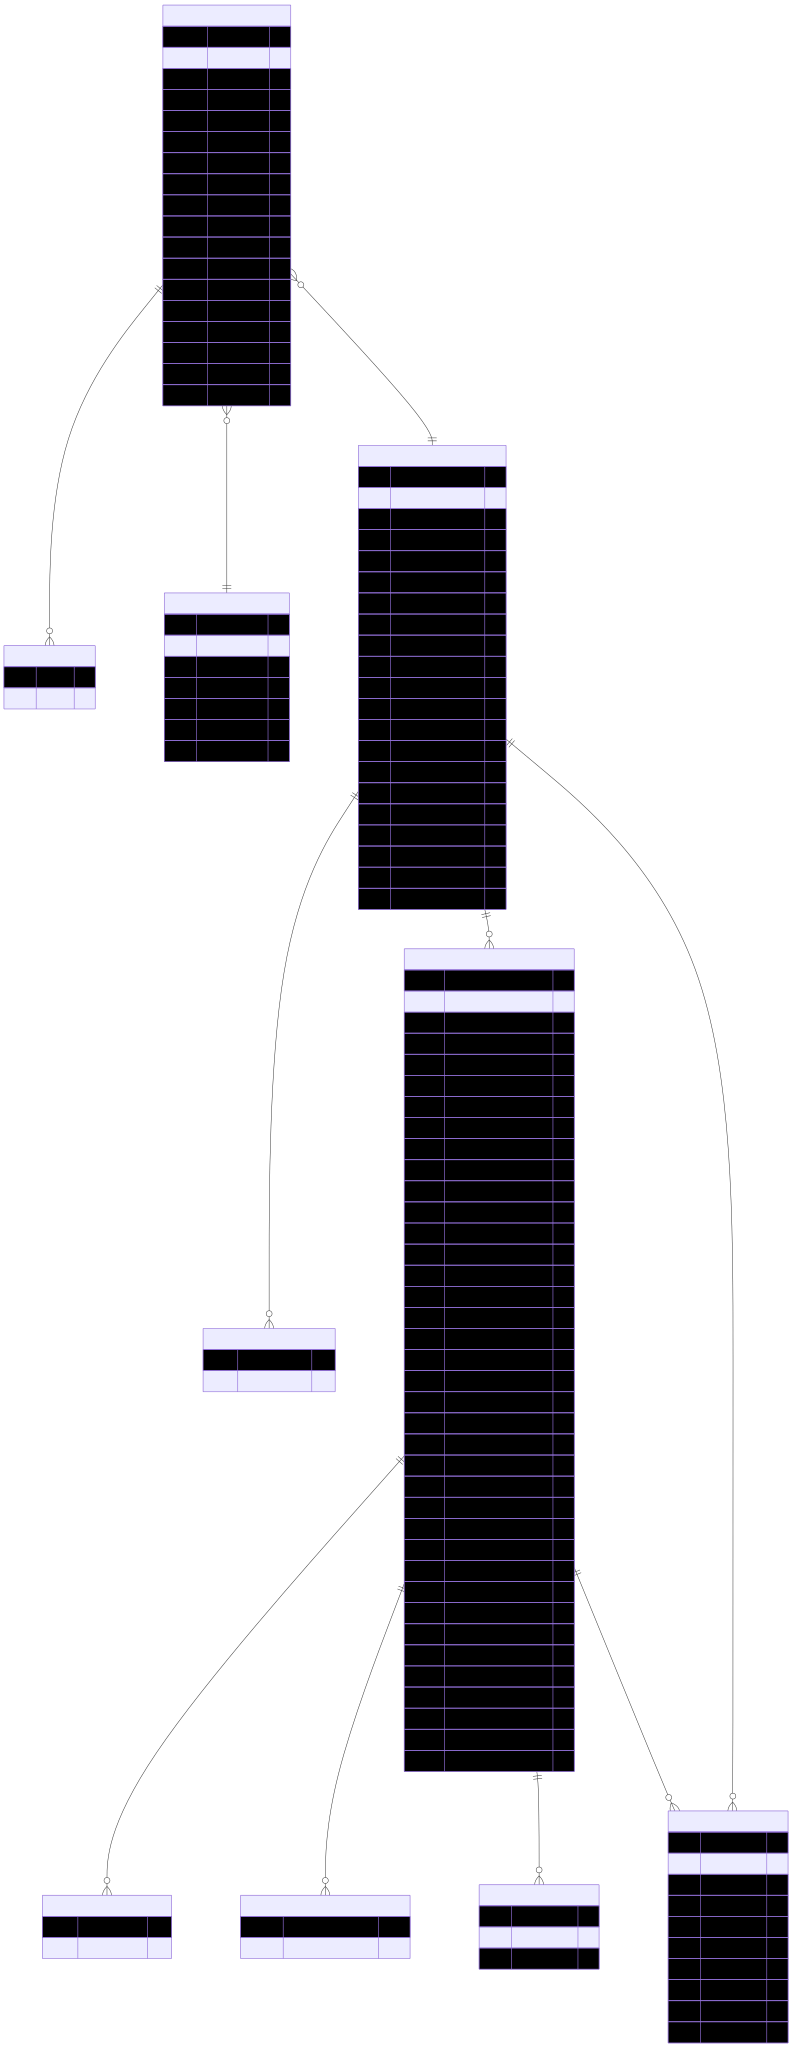
\includegraphics[width=0.9\textwidth]{ERD.png}
\caption{Diagramme d'entités relationnelles de SecuCom}
\end{figure}

Les principales entités de la base de données sont :

\begin{itemize}
  \item \textbf{TUSER} : Stocke les informations de base des utilisateurs (identifiant, email, mot de passe, nom, prénom, etc.). Cette table utilise l'héritage par une colonne discriminante (DTYPE) pour distinguer les différents types d'utilisateurs.

  \item \textbf{USER\_ROLES} : Table de jointure qui associe les utilisateurs à leurs rôles.

  \item \textbf{TSOCIAL\_SECRETARIAT} : Stocke les informations des secrétariats sociaux (nom, numéro d'entreprise, adresse, téléphone, email, site web).

  \item \textbf{TCOMPANY} : Stocke les informations des entreprises clientes (nom, téléphone, email, IBAN, numéro BCE, numéro ONSS, forme juridique, etc.).

  \item \textbf{COMPANY\_JOINT\_COMMITTEES} : Stocke les commissions paritaires associées aux entreprises.

  \item \textbf{TCOLLABORATOR} : Stocke les informations des travailleurs des entreprises clientes (nom, prénom, nationalité, date de naissance, lieu de naissance, genre, langue, état civil, numéro national, fonction, type de contrat, régime de travail, salaire, etc.).

  \item \textbf{COLLABORATOR\_DEPENDENTS} : Stocke les personnes à charge des collaborateurs.

  \item \textbf{COLLABORATOR\_EXTRA\_LEGAL\_BENEFITS} : Stocke les avantages extra-légaux des collaborateurs.

  \item \textbf{COLLABORATOR\_SCHEDULE} : Stocke les horaires de travail des collaborateurs.

  \item \textbf{TDIMONA} : Stocke les informations des déclarations DIMONA (type, date d'entrée, date de sortie, raison de sortie, statut, référence ONSS, message d'erreur, etc.).
\end{itemize}

Les relations entre ces entités sont les suivantes :

\begin{itemize}
  \item Un utilisateur peut avoir plusieurs rôles (relation one-to-many entre TUSER et USER\_ROLES).
  \item Un utilisateur peut être associé à un secrétariat social (relation many-to-one entre TUSER et TSOCIAL\_SECRETARIAT).
  \item Un utilisateur peut être associé à une entreprise (relation many-to-one entre TUSER et TCOMPANY).
  \item Une entreprise peut avoir plusieurs commissions paritaires (relation one-to-many entre TCOMPANY et COMPANY\_JOINT\_COMMITTEES).
  \item Une entreprise peut avoir plusieurs collaborateurs (relation one-to-many entre TCOMPANY et TCOLLABORATOR).
  \item Une entreprise peut avoir plusieurs déclarations DIMONA (relation one-to-many entre TCOMPANY et TDIMONA).
  \item Un collaborateur peut avoir plusieurs personnes à charge (relation one-to-many entre TCOLLABORATOR et COLLABORATOR\_DEPENDENTS).
  \item Un collaborateur peut avoir plusieurs avantages extra-légaux (relation one-to-many entre TCOLLABORATOR et COLLABORATOR\_EXTRA\_LEGAL\_BENEFITS).
  \item Un collaborateur peut avoir plusieurs horaires de travail (relation one-to-many entre TCOLLABORATOR et COLLABORATOR\_SCHEDULE).
  \item Un collaborateur peut avoir plusieurs déclarations DIMONA (relation one-to-many entre TCOLLABORATOR et TDIMONA).
\end{itemize}

\textbf{Champs obligatoires (NOT NULL):}
\begin{itemize}
  \item USER: firstName, lastName, username, email, password, roles, createdAt, accountStatus
  \item SOCIAL\_SECRETARIAT: name, companyNumber
  \item COMPANY: name
  \item COLLABORATOR: lastName, firstName, serviceEntryDate, company\_id, createdAt
  \item DIMONA: collaborator\_id, company\_id
\end{itemize}

\textbf{Contraintes d'unicité (UNIQUE):}
\begin{itemize}
  \item USER: username, email
  \item COMPANY: bceNumber, onssNumber, vatNumber
  \item COLLABORATOR: nationalNumber
\end{itemize}

\textbf{Types énumérés:}
\begin{itemize}
  \item USER.accountStatus: ACTIVE (défaut), INACTIVE, LOCKED, PENDING
  \item COLLABORATOR.type: EMPLOYEE, WORKER, FREELANCE, INTERN, STUDENT
  \item COLLABORATOR.workDurationType: FIXED, VARIABLE
\end{itemize}

Ce modèle de données permet de représenter efficacement les relations complexes entre les différentes entités du système, tout en assurant l'intégrité des données et la performance des requêtes.

\section{Diagrammes de séquences}

Les diagrammes de séquence ci-dessous illustrent les interactions entre les différents composants du système pour les cas d'utilisation clés.

\subsection{Cas d'utilisation : Création d'une entreprise}

Le diagramme de séquence ci-dessous illustre le processus de création d'une entreprise dans le système SecuCom. Ce processus implique trois acteurs principaux : l'Administrateur, le Contact Entreprise et l'Employé du Secrétariat Social.

\begin{figure}[h]
\centering
\includegraphics[width=0.9\textwidth]{SD_creation_entreprise.png}
\caption{Diagramme de séquence - Création d'une entreprise}
\end{figure}

\subsubsection{Description du processus}

\begin{enumerate}
  \item \textbf{Initialisation par l'Administrateur} :
    \begin{itemize}
      \item L'Administrateur crée un compte utilisateur de type "company" avec les données minimales obligatoires.
      \item Le système enregistre ces informations dans la base de données et confirme la création du compte.
    \end{itemize}

  \item \textbf{Transmission des identifiants} :
    \begin{itemize}
      \item L'Administrateur transmet les identifiants de connexion au Contact Entreprise (cette étape se déroule en dehors du système, par exemple par email ou téléphone).
    \end{itemize}

  \item \textbf{Complétion des informations par le Contact Entreprise} :
    \begin{itemize}
      \item Le Contact Entreprise se connecte au système avec les identifiants fournis.
      \item Le système affiche un formulaire permettant de compléter les informations de l'entreprise.
      \item Le Contact Entreprise saisit et soumet les informations complètes de son entreprise (nom, numéro BCE, numéro ONSS, numéro TVA, etc.).
      \item Le système valide les données soumises.
    \end{itemize}

  \item \textbf{Traitement des données} :
    \begin{itemize}
      \item Si les données sont valides, le système les enregistre dans la base de données et confirme l'enregistrement au Contact Entreprise.
      \item Si les données sont invalides, le système affiche les erreurs de validation au Contact Entreprise, qui doit les corriger et soumettre à nouveau.
    \end{itemize}

  \item \textbf{Accès par le Secrétariat Social} :
    \begin{itemize}
      \item L'Employé du Secrétariat Social peut accéder aux informations de l'entreprise.
      \item Le système récupère ces informations depuis la base de données et les affiche à l'Employé du Secrétariat Social.
    \end{itemize}
\end{enumerate}

\subsubsection{Avantages de cette approche}

Cette approche de création d'entreprise présente plusieurs avantages :
\begin{itemize}
  \item Elle responsabilise le Contact Entreprise pour la fourniture et la maintenance de ses propres informations.
  \item Elle réduit la charge administrative pour l'Administrateur et le Secrétariat Social.
  \item Elle améliore la précision des données puisqu'elles sont fournies directement par la source.
  \item Elle s'inscrit dans un modèle de self-service plus moderne et efficace.
  \item Elle facilite la scalabilité du système en permettant de gérer un plus grand nombre d'entreprises.
\end{itemize}

Ce processus constitue la première étape dans le cycle de vie d'une entreprise au sein du système SecuCom, et sert de fondation pour les autres cas d'utilisation comme l'ajout de collaborateurs et la création de déclarations DIMONA.

\subsection{Cas d'utilisation : Ajout d'un collaborateur}

Le diagramme de séquence ci-dessous illustre le processus d'ajout d'un collaborateur (employé) dans le système SecuCom. Ce processus implique plusieurs composants du système et inclut des validations importantes pour garantir l'intégrité des données.

\begin{figure}[h]
\centering
\includegraphics[width=0.9\textwidth]{SD_creation_collaborateur.png}
\caption{Diagramme de séquence - Ajout d'un collaborateur}
\end{figure}

\subsubsection{Description du processus}

\begin{enumerate}
  \item \textbf{Initiation de l'ajout} :
    \begin{itemize}
      \item \textbf{Scénario 1} : Le Contact Entreprise initie l'ajout d'un collaborateur, remplit le formulaire et soumet les données au système.
      \item \textbf{Scénario 2} : Le Secrétariat Social initie l'ajout d'un collaborateur, remplit le formulaire et soumet les données au système.
    \end{itemize}

  \item \textbf{Enregistrement des données} :
    \begin{itemize}
      \item Le système enregistre directement les informations du collaborateur dans la base de données.
      \item Une confirmation est envoyée à l'initiateur de la demande.
    \end{itemize}

  \item \textbf{Notification} :
    \begin{itemize}
      \item L'autre partie (celle qui n'a pas initié l'ajout) est notifiée de l'ajout du collaborateur.
      \item Elle peut consulter les détails du collaborateur ajouté.
    \end{itemize}
\end{enumerate}

\subsubsection{Aspects importants du processus}

Ce processus met en évidence plusieurs aspects importants du système SecuCom :

\begin{itemize}
  \item \textbf{Double flux d'initiation} : La flexibilité du système permet à deux types d'acteurs différents d'initier le processus selon les besoins et les préférences.
  \item \textbf{Simplicité du processus} : Le processus est simplifié pour permettre un ajout rapide et efficace des collaborateurs.
  \item \textbf{Communication bidirectionnelle} : Le système sert d'intermédiaire pour la communication entre le Contact Entreprise et le Secrétariat Social, facilitant le partage d'informations.
  \item \textbf{Traçabilité} : Toutes les étapes du processus sont enregistrées dans la base de données, permettant un suivi de l'historique des ajouts de collaborateurs.
\end{itemize}

L'ajout d'un collaborateur est une étape cruciale qui permet ensuite de procéder à d'autres opérations comme la création de déclarations DIMONA pour ce collaborateur.

\subsection{Cas d'utilisation : Création d'une déclaration DIMONA}

Le diagramme de séquence ci-dessous illustre le processus de création d'une déclaration DIMONA dans le système SecuCom. Ce processus peut être initié soit par le Contact Entreprise, soit par le Secrétariat Social, et implique une validation manuelle des données avant la soumission à l'ONSS.

\begin{figure}[h]
\centering
\includegraphics[width=0.9\textwidth]{SD_creation_dimona.png}
\caption{Diagramme de séquence - Création d'une déclaration DIMONA}
\end{figure}

\subsubsection{Description du processus}

\begin{enumerate}
  \item \textbf{Initiation de la demande} :
    \begin{itemize}
      \item \textbf{Scénario 1} : Le Contact Entreprise initie la création d'une déclaration DIMONA, remplit le formulaire et soumet les données au système.
      \item \textbf{Scénario 2} : Le Secrétariat Social initie la création d'une déclaration DIMONA, remplit le formulaire et soumet les données au système.
    \end{itemize}

  \item \textbf{Notification} :
    \begin{itemize}
      \item L'autre partie (celle qui n'a pas initié la demande) est notifiée de la nouvelle demande DIMONA.
      \item Elle peut consulter les détails de la demande.
    \end{itemize}

  \item \textbf{Création sur le site de l'ONSS} :
    \begin{itemize}
      \item Le Secrétariat Social crée la déclaration DIMONA sur le site officiel de l'ONSS.
    \end{itemize}

  \item \textbf{Traitement du résultat} :
    \begin{itemize}
      \item \textbf{Si la DIMONA est acceptée par l'ONSS} :
        \begin{itemize}
          \item L'ONSS confirme la création de la DIMONA.
          \item Le Secrétariat Social met à jour le statut dans le système.
          \item Le Contact Entreprise est notifié de la création effective de la DIMONA.
        \end{itemize}
      \item \textbf{Si la DIMONA est refusée ou les données sont insuffisantes} :
        \begin{itemize}
          \item L'ONSS refuse la DIMONA ou signale que les données sont insuffisantes.
          \item Le Secrétariat Social change le statut de la demande en "à corriger".
          \item Le Contact Entreprise est notifié et doit modifier les données.
          \item Après correction, le Secrétariat Social est notifié et fait une nouvelle tentative sur le site de l'ONSS.
          \item Une fois la DIMONA acceptée, le statut est mis à jour et le Contact Entreprise est notifié.
        \end{itemize}
    \end{itemize}
\end{enumerate}

\subsubsection{Aspects importants du processus}

Ce processus met en évidence plusieurs aspects importants du système SecuCom :

\begin{itemize}
  \item \textbf{Double flux d'initiation} : La flexibilité du système permet à deux types d'acteurs différents d'initier le processus selon les besoins et les préférences.
  \item \textbf{Gestion des refus et corrections} : Le système permet de gérer les cas où la DIMONA est refusée par l'ONSS, avec un mécanisme de notification et de correction.
  \item \textbf{Communication bidirectionnelle} : Le système sert d'intermédiaire pour la communication entre le Contact Entreprise et le Secrétariat Social.
  \item \textbf{Intégration avec les systèmes externes} : Le processus inclut l'interaction avec le site officiel de l'ONSS pour la création effective de la déclaration.
  \item \textbf{Traçabilité} : Le système maintient un suivi du statut des déclarations DIMONA, permettant aux parties concernées de connaître l'état actuel de chaque déclaration.
\end{itemize}

La création d'une déclaration DIMONA représente l'aboutissement du processus de gestion des collaborateurs, permettant de déclarer officiellement leur engagement auprès des autorités compétentes.

% \section{Diagramme d'activité}

% Le diagramme d'activité ci-dessous illustre le flux de travail typique pour la gestion d'un collaborateur dans le système SecuCom, depuis sa création jusqu'à la génération de sa fiche de paie.

% Ce flux de travail comprend plusieurs étapes :
% \begin{enumerate}
%   \item Création de l'entreprise cliente
%   \item Ajout d'un contact pour l'entreprise
%   \item Ajout d'un collaborateur à l'entreprise
%   \item Création d'une déclaration DIMONA pour le collaborateur
%   \item Suivi du statut de la déclaration DIMONA, qui peut être :
%      \begin{itemize}
%        \item En attente
%        \item Acceptée
%        \item Rejetée (nécessitant une correction et une nouvelle soumission)
%      \end{itemize}
%   \item Enregistrement des prestations du collaborateur
%   \item Génération de la fiche de paie
%   \item Archivage et envoi des documents
% \end{enumerate}

% Chaque étape du flux peut être réalisée par différents acteurs (employé du secrétariat, contact d'entreprise) selon leurs permissions dans le système. Le flux n'est pas strictement linéaire et peut comporter des boucles ou des branches conditionnelles selon les besoins spécifiques de chaque cas.

% Ce diagramme d'activité permet de visualiser clairement le processus métier global et d'identifier les points d'interaction entre les différents acteurs et le système.

% Conception
\chapter{Conception}

Cette section présente les choix technologiques qui ont guidé la conception de SecuCom, tant au niveau du frontend que du backend.

\section{Introduction à l'architecture technique}

L'architecture de SecuCom suit un modèle client-serveur avec une séparation claire entre le frontend et le backend. Le système est organisé en plusieurs couches :

\begin{itemize}
  \item \textbf{Couche Présentation} : Interface utilisateur ReactJS communiquant avec le backend via des API REST
  \item \textbf{Couche API} : Contrôleurs REST exposant les fonctionnalités du système
  \item \textbf{Couche Service} : Services métier implémentant la logique fonctionnelle
  \item \textbf{Couche Persistance} : Repositories gérant l'accès aux données via JPA/Hibernate
  \item \textbf{Couche Sécurité} : Composants gérant l'authentification et l'autorisation via JWT
\end{itemize}

Cette architecture en couches permet une séparation claire des responsabilités, facilitant le développement, les tests et la maintenance.

\section{Technologies front-end}

Pour le développement du frontend, plusieurs technologies modernes ont été sélectionnées afin de créer une interface utilisateur intuitive et professionnelle.

\subsection{ReactJS}

ReactJS constitue le cœur du frontend. Je suis particulièrement attiré par ce framework JavaScript largement adopté dans le monde professionnel pour sa philosophie déclarative et son approche basée sur les composants. Ses principaux avantages incluent :

\begin{itemize}
  \item Modèle basé sur les composants facilitant la réutilisation
  \item DOM virtuel optimisant les performances
  \item Écosystème riche et communauté active
  \item Flux de données unidirectionnel simplifiant le débogage
\end{itemize}

\subsection{TypeScript}

TypeScript a été choisi comme surcouche à JavaScript pour apporter un typage statique, améliorant la détection précoce des erreurs et la maintenabilité du code.

\subsection{Tailwind CSS}

Tailwind CSS a été adopté pour son approche "utility-first" offrant une grande flexibilité dans la conception tout en maintenant une cohérence visuelle.

\subsection{shadcnUI}

Cette collection de composants UI réutilisables, construits avec Radix UI et stylisés avec Tailwind CSS, a permis d'accélérer le développement de l'interface tout en garantissant l'accessibilité.

\subsection{React Router DOM}

React Router DOM gère la navigation entre les différentes pages de l'application, offrant une expérience utilisateur fluide sans rechargement complet des pages.

\section{Technologies back-end}

Le backend a été développé avec des technologies robustes centrées autour de l'écosystème Spring.

\subsection{Spring Boot}

Spring Boot constitue le fondement du backend. Je suis littéralement tombé sous le charme de ce framework qui simplifie considérablement le développement d'applications Java grâce à sa configuration automatique et ses conventions judicieuses.

\subsection{Spring Security}

Spring Security gère l'authentification et l'autorisation, offrant une protection contre les attaques courantes et permettant une gestion fine des accès basée sur les rôles.

\subsection{Spring Data JPA}

Cette bibliothèque simplifie l'accès aux données en réduisant le code boilerplate nécessaire pour les opérations CRUD, permettant de se concentrer sur la logique métier.

\subsection{Hibernate}

Utilisé comme implémentation de JPA, Hibernate facilite la traduction entre les objets Java et les tables de la base de données.

\subsection{JSON Web Tokens (JWT)}

Les JWT ont été choisis comme mécanisme d'authentification sans état, facilitant la scalabilité et éliminant le besoin de stocker des sessions côté serveur.

\subsection{Base de données relationnelle}

Une base de données relationnelle a été choisie pour sa capacité à gérer efficacement les relations complexes entre les différentes entités du système.

\section{Pourquoi ces choix ?}

Les choix technologiques ont été guidés par plusieurs critères essentiels :

\subsection{Adéquation aux besoins fonctionnels}

Les technologies choisies répondent parfaitement aux exigences de SecuCom, notamment la création d'une interface intuitive (ReactJS, Tailwind), la gestion de données complexes (Spring Data JPA, Hibernate) et la sécurisation des accès (Spring Security, JWT).

\subsection{Maturité et productivité}

L'écosystème Spring et ReactJS sont des solutions éprouvées avec des communautés actives, offrant un excellent équilibre entre puissance et productivité de développement.

\subsection{Maintenabilité et évolutivité}

L'architecture modulaire et la séparation claire des responsabilités facilitent la maintenance et l'évolution du système, tandis que TypeScript améliore la robustesse du code frontend.

\subsection{Développement professionnel}

Mon attrait personnel pour Spring Boot et ma volonté de maîtriser ReactJS pour créer des interfaces utilisateur professionnelles et réactives ont également influencé ces choix technologiques, me permettant de développer des compétences valorisées sur le marché du travail.

% Développement
\chapter{Développement}

Cette section présente l'implémentation technique de SecuCom, en détaillant l'architecture de l'application, les modèles de données, les contrôleurs et services, ainsi que les fonctionnalités principales et les mécanismes de sécurité.

\section{Architecture de l'application}

\subsection{Vue d'ensemble}

L'implémentation de SecuCom suit une architecture en couches clairement séparées, permettant une meilleure organisation du code, une maintenance facilitée et une évolution plus souple du système. Cette architecture s'articule autour de cinq couches principales :

\begin{itemize}
  \item \textbf{Couche Modèle} : Représente les entités métier et leurs relations, implémentée via des classes Java annotées avec JPA.
  \item \textbf{Couche Repository} : Fournit les mécanismes d'accès aux données via Spring Data JPA, permettant d'abstraire les opérations de persistance.
  \item \textbf{Couche Service} : Contient la logique métier de l'application, orchestrant les opérations entre les repositories et les contrôleurs.
  \item \textbf{Couche DTO} : Assure la transformation des données entre la couche service et la couche contrôleur, permettant de découpler les modèles internes des représentations externes.
  \item \textbf{Couche Contrôleur} : Expose les API REST qui permettent aux clients (frontend) d'interagir avec le système.
\end{itemize}

Cette architecture est complétée par une couche transversale de sécurité qui gère l'authentification et l'autorisation à travers toutes les couches de l'application.

\begin{figure}[h]
\centering
% Placeholder for a diagram - you might want to create and include an actual diagram here
\caption{Architecture en couches de SecuCom}
\end{figure}

Le flux de données typique dans l'application suit le parcours suivant :

\begin{enumerate}
  \item Le client (frontend) envoie une requête HTTP à un endpoint REST.
  \item La requête traverse d'abord la couche de sécurité qui vérifie l'authentification et les autorisations.
  \item Le contrôleur approprié reçoit la requête, valide les données d'entrée et les transmet au service correspondant.
  \item Le service applique la logique métier nécessaire et interagit avec les repositories pour accéder aux données.
  \item Les repositories communiquent avec la base de données via JPA/Hibernate.
  \item Le résultat remonte la chaîne : repository → service → contrôleur, avec les transformations DTO appropriées.
  \item Le contrôleur renvoie une réponse HTTP formatée au client.
\end{enumerate}

Cette séparation des responsabilités permet non seulement une meilleure organisation du code, mais facilite également les tests unitaires et d'intégration, chaque couche pouvant être testée indépendamment.

\subsubsection{Organisation du frontend}

Le frontend de SecuCom est divisé en deux espaces distincts correspondant aux deux principaux rôles d'utilisateurs :

\begin{itemize}
  \item \textbf{Espace Secrétariat Social} : Accessible aux utilisateurs ayant le rôle \texttt{ROLE\_SECRETARIAT}, cet espace permet la gestion de toutes les entreprises clientes, leurs collaborateurs et leurs déclarations DIMONA.
  \item \textbf{Espace Entreprise} : Accessible aux utilisateurs ayant le rôle \texttt{ROLE\_COMPANY}, cet espace est limité aux données de l'entreprise à laquelle l'utilisateur est associé.
\end{itemize}

Cette séparation est implémentée au niveau du routage dans l'application React, avec des routes protégées qui vérifient le rôle de l'utilisateur avant d'autoriser l'accès. Bien que les deux espaces soient distincts en termes de données accessibles, ils partagent la même interface utilisateur (UI) pour maintenir une expérience cohérente. Les composants React sont réutilisés entre les deux espaces, mais les données affichées sont filtrées en fonction du rôle de l'utilisateur.

Par exemple, le même composant de liste de collaborateurs est utilisé dans les deux espaces, mais dans l'espace Secrétariat Social, il peut afficher les collaborateurs de toutes les entreprises (avec possibilité de filtrer par entreprise), tandis que dans l'espace Entreprise, il n'affiche que les collaborateurs de l'entreprise de l'utilisateur connecté.

\subsection{Modèles de données}

Les modèles de données constituent le cœur de l'application SecuCom. Ils représentent les entités métier et leurs relations, et sont implémentés sous forme de classes Java annotées avec JPA (Java Persistence API) pour la persistance en base de données.

\subsubsection{Entité User}

L'entité \texttt{User} représente la base de tous les utilisateurs du système. Elle utilise l'héritage avec une stratégie de table unique (\texttt{SINGLE\_TABLE}) pour différencier les types d'utilisateurs via une colonne discriminante.

\begin{lstlisting}
@Entity
@Table(name = "TUser")
@Inheritance(strategy = InheritanceType.SINGLE_TABLE)
@DiscriminatorColumn(name = "DTYPE")
@DiscriminatorValue("User")
public class User {
    @Id
    @GeneratedValue(strategy = GenerationType.UUID)
    private UUID id;
    
    private String firstName;
    private String lastName;
    private String username;
    private String email;
    private String password;
    
    @ElementCollection(fetch = FetchType.EAGER)
    @Enumerated(EnumType.STRING)
    private Set<Role> roles = new HashSet<>();
    
    // Autres attributs et methodes
}
\end{lstlisting}

Cette approche d'héritage permet de spécialiser les utilisateurs en différents types (employés du secrétariat, contacts d'entreprise) tout en maintenant une base commune pour l'authentification et les informations de base.

\subsubsection{Entité Company}

L'entité \texttt{Company} représente une entreprise cliente du secrétariat social. Elle contient de nombreux attributs reflétant les informations administratives et légales nécessaires.

\begin{lstlisting}
@Entity
@Table(name = "TCompany")
public class Company {
    @Id
    @GeneratedValue(strategy = GenerationType.UUID)
    private UUID id;
    
    @Column(nullable = false)
    private String name;
    
    @Column(unique = true)
    private String bceNumber;
    
    @Column(unique = true)
    private String onssNumber;
    
    @OneToMany(mappedBy = "company", cascade = CascadeType.ALL)
    private Set<Collaborator> collaborators = new HashSet<>();
    
    // Autres attributs et methodes
}
\end{lstlisting}

Cette entité est au centre de nombreuses relations : elle est liée aux contacts d'entreprise, aux collaborateurs et aux déclarations DIMONA.

\subsubsection{Entité Collaborator}

L'entité \texttt{Collaborator} représente un travailleur d'une entreprise cliente. Elle contient des informations personnelles et professionnelles détaillées.

\begin{lstlisting}
@Entity
@Table(name = "TCollaborator")
public class Collaborator {
    @Id
    @GeneratedValue(strategy = GenerationType.UUID)
    private UUID id;
    
    private String lastName;
    private String firstName;
    private String nationality;
    private LocalDate birthDate;
    
    @Size(max = 20)
    @Column(name = "national_number", unique = true)
    private String nationalNumber;
    
    @ManyToOne(fetch = FetchType.LAZY)
    @JoinColumn(name = "company_id", nullable = false)
    private Company company;
    
    // Autres attributs et methodes
}
\end{lstlisting}

Cette entité utilise des types énumérés pour certains attributs comme le type de collaborateur (\texttt{EMPLOYEE}, \texttt{WORKER}, etc.) et le type de durée de travail (\texttt{FIXED}, \texttt{VARIABLE}).

\subsubsection{Entité Dimona}

L'entité \texttt{Dimona} représente une déclaration DIMONA associée à un collaborateur et à une entreprise.

\begin{lstlisting}
@Entity
@Table(name = "TDimona")
public class Dimona {
    @Id
    @GeneratedValue(strategy = GenerationType.UUID)
    private UUID id;
    
    private String type;
    private Date entryDate;
    private Date exitDate;
    private String status;
    private String onssReference;
    
    @ManyToOne(fetch = FetchType.EAGER)
    @JoinColumn(name = "collaborator_id", nullable = false)
    private Collaborator collaborator;
    
    @ManyToOne(fetch = FetchType.EAGER)
    @JoinColumn(name = "company_id", nullable = false)
    private Company company;
    
    // Autres attributs et methodes
}
\end{lstlisting}

Cette entité permet de suivre l'état des déclarations DIMONA et de conserver les références attribuées par l'ONSS.

\subsubsection{Autres entités et relations}

Le modèle de données comprend également d'autres entités comme \texttt{Address} (utilisée comme classe embarquée dans plusieurs entités), \texttt{SocialSecretariat} (représentant le secrétariat social) et \texttt{SecretariatEmployee} (représentant un employé du secrétariat social).

Les relations entre ces entités sont soigneusement définies pour refléter la réalité métier :
\begin{itemize}
  \item Une entreprise peut avoir plusieurs contacts et plusieurs collaborateurs (relations one-to-many).
  \item Un collaborateur appartient à une seule entreprise (relation many-to-one).
  \item Une déclaration DIMONA est associée à un collaborateur et à une entreprise (relations many-to-one).
  \item Un utilisateur peut avoir plusieurs rôles (relation one-to-many avec une collection d'énumérations).
\end{itemize}

Cette modélisation riche permet de représenter fidèlement les concepts métier tout en facilitant les requêtes et les manipulations de données.

\subsection{Contrôleurs et services}

L'architecture de SecuCom s'appuie sur une séparation claire entre les contrôleurs, qui exposent les API REST, et les services, qui implémentent la logique métier. Cette séparation permet une meilleure organisation du code et facilite les tests.

\subsubsection{Contrôleurs REST}

Les contrôleurs REST sont responsables de la gestion des requêtes HTTP, de la validation des données d'entrée et de la transformation des réponses. Ils sont annotés avec \texttt{@RestController} et définissent des endpoints accessibles via des methodes HTTP (GET, POST, PUT, DELETE).

Voici un exemple avec le contrôleur de gestion des entreprises :

\begin{lstlisting}
@RestController
@RequestMapping("/company")
public class CompanyController {
    private final CompanyService companyService;
    
    public CompanyController(CompanyService companyService) {
        this.companyService = companyService;
    }
    
    @PostMapping
    public ResponseEntity<CompanyDto> createCompany(
            @Valid @RequestBody CompanyDto companyDto) {
        CompanyDto createdCompany = companyService.createCompany(companyDto);
        return new ResponseEntity<>(createdCompany, HttpStatus.CREATED);
    }
    
    @GetMapping("/{id}")
    public ResponseEntity<CompanyDto> getCompanyById(@PathVariable UUID id) {
        CompanyDto company = companyService.getCompanyById(id);
        return ResponseEntity.ok(company);
    }
    
    // Autres methodes
}
\end{lstlisting}

Les contrôleurs utilisent des objets DTO (Data Transfer Object) pour les échanges avec les clients, ce qui permet de découpler les modèles internes des représentations externes.

Les principaux contrôleurs de l'application sont :
\begin{itemize}
  \item \texttt{AuthController} : Gère l'authentification et les tokens JWT.
  \item \texttt{CompanyController} : Gère les opérations CRUD sur les entreprises.
  \item \texttt{CollaboratorController} : Gère les opérations CRUD sur les collaborateurs.
  \item \texttt{DimonaController} : Gère les opérations liées aux déclarations DIMONA.
  \item \texttt{UserController} : Gère les opérations sur les utilisateurs.
  \item \texttt{SocialSecretariatController} : Gère les opérations liées au secrétariat social.
\end{itemize}

\subsubsection{Services métier}

Les services métier encapsulent la logique fonctionnelle de l'application. Ils orchestrent les opérations entre les repositories et les contrôleurs, appliquent les règles métier et gèrent les transactions.

Voici un exemple simplifié de service pour la gestion des entreprises :

\begin{lstlisting}
@Service
@Transactional
public class CompanyService {
    private final CompanyRepository companyRepository;
    private final ModelMapper modelMapper;
    
    public CompanyService(CompanyRepository companyRepository, 
                         ModelMapper modelMapper) {
        this.companyRepository = companyRepository;
        this.modelMapper = modelMapper;
    }
    
    public CompanyDto createCompany(CompanyDto companyDto) {
        // Verification des donnees
        if (companyRepository.existsByBceNumber(companyDto.getBceNumber())) {
            throw new RuntimeException("BCE number already exists");
        }
        
        // Conversion DTO -> Entity
        Company company = modelMapper.map(companyDto, Company.class);
        
        // Persistance
        Company savedCompany = companyRepository.save(company);
        
        // Conversion Entity -> DTO pour la reponse
        return modelMapper.map(savedCompany, CompanyDto.class);
    }
    
    // Autres methodes
}
\end{lstlisting}

Les services utilisent l'annotation \texttt{@Transactional} pour gérer les transactions de manière déclarative, assurant l'intégrité des données même en cas d'erreur.

Les principaux services de l'application sont :
\begin{itemize}
  \item \texttt{AuthService} : Gère l'authentification et la génération des tokens.
  \item \texttt{CompanyService} : Implémente la logique métier pour les entreprises.
  \item \texttt{CollaboratorService} : Implémente la logique métier pour les collaborateurs.
  \item \texttt{DimonaService} : Implémente la logique métier pour les déclarations DIMONA.
  \item \texttt{UserService} : Implémente la logique métier pour les utilisateurs.
  \item \texttt{SocialSecretariatService} : Implémente la logique métier pour le secrétariat social.
\end{itemize}

\subsubsection{Repositories}

Les repositories fournissent une abstraction de l'accès aux données. Ils sont implémentés en utilisant Spring Data JPA, qui génère automatiquement les implémentations à partir d'interfaces.

\begin{lstlisting}
public interface CompanyRepository extends JpaRepository<Company, UUID> {
    boolean existsByBceNumber(String bceNumber);
    boolean existsByOnssNumber(String onssNumber);
    boolean existsByVatNumber(String vatNumber);
    // Autres methodes
}
\end{lstlisting}

Cette approche permet de réduire considérablement le code boilerplate tout en offrant des fonctionnalités puissantes comme le filtrage, le tri et la pagination.

\subsubsection{DTOs (Data Transfer Objects)}

Les DTOs sont utilisés pour découpler les modèles internes des représentations externes. Ils permettent de :
\begin{itemize}
  \item Contrôler précisément les données exposées aux clients
  \item Valider les données d'entrée indépendamment des entités
  \item Adapter le format des données aux besoins spécifiques des clients
\end{itemize}

\begin{lstlisting}
@Data
@NoArgsConstructor
@AllArgsConstructor
public class CompanyDto {
    private UUID id;
    
    @NotBlank
    @Size(max = 100)
    private String name;
    
    @Pattern(regexp = "^[0-9]{10}$")
    private String bceNumber;
    
    @Pattern(regexp = "^[0-9]{9}$")
    private String onssNumber;
    
    // Autres attributs
}
\end{lstlisting}

La conversion entre DTOs et entités est généralement gérée par des bibliothèques comme ModelMapper ou MapStruct, ou par des methodes de conversion manuelles dans les services.

\section{Fonctionnalités principales}

\subsection{Gestion des entreprises}

La gestion des entreprises est une fonctionnalité centrale de SecuCom, permettant au secrétariat social de gérer efficacement ses clients. Cette fonctionnalité est implémentée à travers plusieurs composants qui travaillent ensemble.

\subsubsection{Modèle de données}

Le modèle de données pour les entreprises est centré autour de l'entité \texttt{Company}, qui stocke toutes les informations nécessaires :

\begin{itemize}
  \item Informations d'identification : nom, numéro BCE, numéro ONSS, numéro TVA
  \item Informations de contact : téléphone, email, adresse
  \item Informations bancaires : IBAN
  \item Informations légales : forme juridique, secteur d'activité, commissions paritaires
  \item Informations de collaboration : date de début, formule souscrite, fréquence de déclaration
\end{itemize}

Cette entité est liée à d'autres entités importantes :
\begin{itemize}
  \item \texttt{CompanyContact} : Utilisateurs ayant accès aux données de l'entreprise
  \item \texttt{Collaborator} : Travailleurs de l'entreprise
  \item \texttt{Dimona} : Déclarations DIMONA associées à l'entreprise
\end{itemize}

\subsubsection{API REST}

L'API REST pour la gestion des entreprises est exposée par le \texttt{CompanyController}, qui offre les endpoints suivants :

\begin{itemize}
  \item \texttt{POST /company} : Création d'une nouvelle entreprise
  \item \texttt{GET /company/\{id\}} : Récupération des détails d'une entreprise
  \item \texttt{GET /company} : Récupération de la liste des entreprises
  \item \texttt{PUT /company/\{id\}} : Mise à jour des informations d'une entreprise
  \item \texttt{DELETE /company/\{id\}} : Suppression d'une entreprise
  \item \texttt{GET /company/check/bce/\{bceNumber\}} : Vérification de l'existence d'un numéro BCE
  \item \texttt{GET /company/check/onss/\{onssNumber\}} : Vérification de l'existence d'un numéro ONSS
  \item \texttt{GET /company/check/vat/\{vatNumber\}} : Vérification de l'existence d'un numéro TVA
\end{itemize}

Ces endpoints sont sécurisés et accessibles uniquement aux utilisateurs autorisés (administrateurs et employés du secrétariat social).

\subsubsection{Logique métier}

La logique métier pour la gestion des entreprises est implémentée dans le \texttt{CompanyService}, qui offre les fonctionnalités suivantes :

\begin{itemize}
  \item Validation des données d'entreprise (unicité des numéros BCE, ONSS et TVA)
  \item Création et mise à jour des entreprises avec gestion des relations
  \item Récupération des entreprises avec filtrage et pagination
  \item Suppression des entreprises avec gestion des dépendances
\end{itemize}

Le service implémente également des règles métier spécifiques, comme la vérification de la validité des numéros BCE et ONSS selon les formats belges.

\subsubsection{Gestion des contacts d'entreprise}

La gestion des contacts d'entreprise est une fonctionnalité complémentaire qui permet de définir quels utilisateurs ont accès aux données d'une entreprise. Elle est implémentée à travers le \texttt{CompanyContactService} et le \texttt{CompanyContactController}.

Les contacts d'entreprise sont des utilisateurs spécialisés (héritant de \texttt{User}) qui ont le rôle \texttt{ROLE\_COMPANY} et sont associés à une entreprise spécifique. Ils peuvent accéder uniquement aux données de leur propre entreprise.

\subsection{Gestion des collaborateurs}

La gestion des collaborateurs est une autre fonctionnalité clé de SecuCom, permettant de gérer les travailleurs des entreprises clientes (qu'ils soient employés, ouvriers, freelances, stagiaires ou étudiants). Cette fonctionnalité est particulièrement importante car elle sert de base pour les déclarations DIMONA.

\subsubsection{Modèle de données}

Le modèle de données pour les collaborateurs est centré autour de l'entité \texttt{Collaborator}, qui stocke de nombreuses informations :

\begin{itemize}
  \item Informations personnelles : nom, prénom, nationalité, date de naissance, lieu de naissance, genre, langue, état civil
  \item Informations d'identification : numéro national (unique)
  \item Informations professionnelles : date d'entrée en service, fonction, type de contrat, régime de travail
  \item Informations de rémunération : salaire, avantages extra-légaux
  \item Informations bancaires : IBAN pour le versement du salaire
\end{itemize}

L'entité \texttt{Collaborator} utilise plusieurs types énumérés pour catégoriser les collaborateurs :
\begin{itemize}
  \item \texttt{CollaboratorType} : EMPLOYEE, WORKER, FREELANCE, INTERN, STUDENT
  \item \texttt{WorkDurationType} : FIXED, VARIABLE
  \item \texttt{Day} : MONDAY, TUESDAY, WEDNESDAY, THURSDAY, FRIDAY, SATURDAY, SUNDAY (pour les horaires)
\end{itemize}

Elle utilise également des classes embarquées comme \texttt{Address} pour structurer les informations d'adresse.

\subsubsection{API REST}

L'API REST pour la gestion des collaborateurs est exposée par le \texttt{CollaboratorController}, qui offre les endpoints suivants :

\begin{itemize}
  \item \texttt{POST /collaborators} : Création d'un nouveau collaborateur
  \item \texttt{GET /collaborators/\{id\}} : Récupération des détails d'un collaborateur
  \item \texttt{GET /collaborators} : Récupération de la liste des collaborateurs
  \item \texttt{GET /collaborators/company/\{companyId\}} : Récupération des collaborateurs d'une entreprise
  \item \texttt{PUT /collaborators/\{id\}} : Mise à jour des informations d'un collaborateur
  \item \texttt{DELETE /collaborators/\{id\}} : Suppression d'un collaborateur
\end{itemize}

Ces endpoints sont sécurisés et accessibles aux utilisateurs autorisés, avec des restrictions basées sur les rôles et les associations d'entreprise.

\subsubsection{Logique métier}

La logique métier pour la gestion des collaborateurs est implémentée dans le \texttt{CollaboratorService}, qui offre les fonctionnalités suivantes :

\begin{itemize}
  \item Validation des données de collaborateur (unicité du numéro national, validité des dates)
  \item Création et mise à jour des collaborateurs avec gestion des relations
  \item Récupération des collaborateurs avec filtrage par entreprise
  \item Suppression des collaborateurs avec gestion des dépendances (déclarations DIMONA)
\end{itemize}

Le service implémente également des règles métier spécifiques, comme la vérification de la validité du numéro national selon le format belge et la gestion des horaires de travail selon le type de durée de travail (fixe ou variable).

\subsubsection{Validation des données}

La validation des données de collaborateur est particulièrement importante en raison des exigences légales pour les déclarations DIMONA. Elle est implémentée à plusieurs niveaux :

\begin{itemize}
  \item Validation des DTOs avec les annotations Jakarta Validation (\texttt{@NotNull}, \texttt{@Size}, \texttt{@Pattern}, etc.)
  \item Validation métier dans le service (cohérence des dates, validité du numéro national)
  \item Contraintes de base de données (unicité du numéro national)
\end{itemize}

Cette approche multi-niveaux garantit l'intégrité et la validité des données de collaborateur, réduisant ainsi les risques d'erreur lors des déclarations officielles.

\subsection{Gestion des déclarations DIMONA}

La gestion des déclarations DIMONA est une fonctionnalité critique de SecuCom, permettant de suivre les déclarations d'emploi auprès de l'ONSS. Cette fonctionnalité est essentielle pour la conformité légale des entreprises clientes.

\subsubsection{Modèle de données}

Le modèle de données pour les déclarations DIMONA est centré autour de l'entité \texttt{Dimona}, qui stocke les informations suivantes :

\begin{itemize}
  \item Type de déclaration (entrée en service, sortie de service)
  \item Dates d'entrée et de sortie
  \item Raison de sortie (si applicable)
  \item Statut de la déclaration (en attente, acceptée, rejetée)
  \item Référence ONSS (attribuée par l'ONSS après acceptation)
  \item Message d'erreur (en cas de rejet)
\end{itemize}

L'entité \texttt{Dimona} est liée à deux autres entités importantes :
\begin{itemize}
  \item \texttt{Collaborator} : Le travailleur concerné par la déclaration
  \item \texttt{Company} : L'entreprise employeuse
\end{itemize}

Cette double association permet de retrouver facilement les déclarations par collaborateur ou par entreprise.

\subsubsection{API REST}

L'API REST pour la gestion des déclarations DIMONA est exposée par le \texttt{DimonaController}, qui offre les endpoints suivants :

\begin{itemize}
  \item \texttt{POST /dimona} : Création d'une nouvelle déclaration DIMONA
  \item \texttt{GET /dimona/\{id\}} : Récupération des détails d'une déclaration
  \item \texttt{GET /dimona} : Récupération de la liste des déclarations
  \item \texttt{GET /dimona/collaborator/\{collaboratorId\}} : Récupération des déclarations d'un collaborateur
  \item \texttt{GET /dimona/company/\{companyId\}} : Récupération des déclarations d'une entreprise
  \item \texttt{DELETE /dimona/\{id\}} : Suppression d'une déclaration
\end{itemize}

Ces endpoints sont sécurisés et accessibles aux utilisateurs autorisés, avec des restrictions basées sur les rôles et les associations d'entreprise.

\subsubsection{Logique métier}

La logique métier pour la gestion des déclarations DIMONA est implémentée dans le \texttt{DimonaService}, qui offre les fonctionnalités suivantes :

\begin{itemize}
  \item Validation des données de déclaration (cohérence des dates, existence du collaborateur et de l'entreprise)
  \item Création des déclarations avec initialisation du statut
  \item Mise à jour du statut des déclarations après traitement par l'ONSS
  \item Récupération des déclarations avec filtrage par collaborateur ou entreprise
\end{itemize}

Le service implémente également des règles métier spécifiques, comme la vérification de la cohérence entre les dates d'entrée et de sortie, et la validation des types de déclaration selon le contexte.

\subsubsection{Processus de déclaration}

Le processus de déclaration DIMONA dans SecuCom est semi-automatisé :

\begin{enumerate}
  \item Un utilisateur (contact d'entreprise ou employé du secrétariat) crée une demande de déclaration DIMONA dans le système.
  \item Le système valide les données et crée une entrée avec le statut "en attente".
  \item Un employé du secrétariat social traite la demande en soumettant manuellement la déclaration sur le site officiel de l'ONSS.
  \item Après traitement par l'ONSS, l'employé met à jour le statut et la référence ONSS dans le système.
  \item Le système notifie le contact d'entreprise du résultat de la déclaration.
\end{enumerate}

Cette approche semi-automatisée permet un contrôle humain sur les déclarations tout en bénéficiant de la validation et du suivi automatisés offerts par le système.

\section{Sécurité et authentification}

La sécurité est un aspect fondamental de SecuCom, étant donné la nature sensible des données traitées. L'application implémente un système robuste d'authentification et d'autorisation basé sur les tokens JWT (JSON Web Tokens).

\subsection{Authentification basée sur JWT}

L'authentification dans SecuCom est implémentée en utilisant les tokens JWT, qui offrent plusieurs avantages :
\begin{itemize}
  \item Authentification sans état (stateless), facilitant la scalabilité
  \item Transmission sécurisée des informations d'identité
  \item Expiration automatique des sessions
  \item Possibilité de révocation des tokens
\end{itemize}

Le processus d'authentification se déroule comme suit :

\begin{enumerate}
  \item L'utilisateur soumet ses identifiants (nom d'utilisateur/email et mot de passe) via l'endpoint \texttt{/auth/login}.
  \item Le système vérifie les identifiants et, s'ils sont valides, génère deux tokens :
    \begin{itemize}
      \item Un token d'accès (access token) de courte durée pour l'authentification
      \item Un token de rafraîchissement (refresh token) de longue durée pour obtenir de nouveaux tokens d'accès
    \end{itemize}
  \item Le token d'accès est renvoyé dans la réponse JSON, tandis que le token de rafraîchissement est stocké dans un cookie HTTP-only sécurisé.
  \item Pour les requêtes ultérieures, le client inclut le token d'accès dans l'en-tête \texttt{Authorization}.
  \item Lorsque le token d'accès expire, le client peut obtenir un nouveau token en utilisant le token de rafraîchissement via l'endpoint \texttt{/auth/refresh}.
\end{enumerate}

Cette implémentation est réalisée à travers plusieurs classes :

\begin{itemize}
  \item \texttt{JwtUtils} : Génère et valide les tokens JWT
  \item \texttt{JwtAuthenticationFilter} : Intercepte les requêtes et extrait les tokens JWT
  \item \texttt{AuthController} : Expose les endpoints d'authentification
  \item \texttt{AuthService} : Implémente la logique d'authentification
  \item \texttt{UserDetailsServiceImpl} : Charge les détails utilisateur pour Spring Security
\end{itemize}

\subsection{Gestion des rôles et autorisations}

SecuCom implémente un système de contrôle d'accès basé sur les rôles (RBAC) en utilisant Spring Security. Trois rôles principaux sont définis :

\begin{itemize}
  \item \texttt{ROLE\_ADMIN} : Administrateurs du système avec accès complet à toutes les fonctionnalités
  \item \texttt{ROLE\_SECRETARIAT} : Employés du secrétariat social avec accès à toutes les entreprises clientes et leurs données
  \item \texttt{ROLE\_COMPANY} : Contacts d'entreprise avec accès limité aux données de leur propre entreprise
\end{itemize}

Ces rôles sont utilisés à plusieurs niveaux pour sécuriser l'application :

\begin{itemize}
  \item \textbf{Niveau URL} : Certains endpoints sont restreints à des rôles spécifiques via la configuration de Spring Security dans \texttt{SecurityConfig}.
  \item \textbf{Niveau méthode} : Des annotations comme \texttt{@PreAuthorize} sont utilisées pour sécuriser des methodes spécifiques dans les contrôleurs et services.
  \item \textbf{Niveau données} : Des filtres sont appliqués dans les services pour limiter l'accès aux données selon le rôle et l'association d'entreprise de l'utilisateur.
\end{itemize}

Par exemple, un utilisateur avec le rôle \texttt{ROLE\_COMPANY} ne peut accéder qu'aux données de sa propre entreprise, tandis qu'un utilisateur avec le rôle \texttt{ROLE\_SECRETARIAT} peut accéder aux données de toutes les entreprises.

\subsection{Sécurisation des communications}

Toutes les communications entre le client et le serveur sont sécurisées via HTTPS/TLS, assurant la confidentialité et l'intégrité des données en transit. La configuration CORS (Cross-Origin Resource Sharing) est également mise en place pour contrôler quels domaines peuvent accéder aux ressources de l'API.

\begin{lstlisting}
@Bean
public CorsConfigurationSource corsConfigurationSource() {
    CorsConfiguration configuration = new CorsConfiguration();
    configuration.setAllowedOrigins(Arrays.asList("http://localhost:5173"));
    configuration.setAllowedMethods(Arrays.asList("GET", "POST", "PUT", "DELETE", "OPTIONS"));
    configuration.setAllowedHeaders(Arrays.asList("*"));
    configuration.setAllowCredentials(true);
    configuration.setMaxAge(3600L);
    UrlBasedCorsConfigurationSource source = new UrlBasedCorsConfigurationSource();
    source.registerCorsConfiguration("/**", configuration);
    return source;
}
\end{lstlisting}

\subsection{Gestion des exceptions de sécurité}

SecuCom implémente une gestion centralisée des exceptions via \texttt{GlobalExceptionHandler}, qui intercepte les exceptions liées à la sécurité et renvoie des réponses appropriées sans exposer de détails sensibles.

\begin{lstlisting}
@ExceptionHandler(AccessDeniedException.class)
public ResponseEntity<ErrorResponse> handleAccessDeniedException(AccessDeniedException ex) {
    ErrorResponse error = new ErrorResponse(
            HttpStatus.FORBIDDEN.value(),
            "Acces refuse",
            "Vous n'avez pas les permissions necessaires pour acceder a cette ressource");
    return new ResponseEntity<>(error, HttpStatus.FORBIDDEN);
}
\end{lstlisting}

Cette approche garantit que les erreurs de sécurité sont traitées de manière cohérente et sécurisée, sans révéler d'informations qui pourraient être exploitées par des attaquants.

\subsection{Protection des mots de passe}

Les mots de passe des utilisateurs sont protégés à l'aide de l'algorithme de hachage BCrypt, qui intègre automatiquement un sel (salt) unique pour chaque mot de passe, rendant les attaques par dictionnaire et par table arc-en-ciel (rainbow table) inefficaces.

\begin{lstlisting}
@Bean
public PasswordEncoder passwordEncoder() {
    return new BCryptPasswordEncoder();
}
\end{lstlisting}

Lors de l'authentification, le mot de passe fourni est haché et comparé au hachage stocké, sans jamais manipuler le mot de passe en clair.

\subsection{Audit et traçabilité}

SecuCom intègre des mécanismes d'audit pour tracer les actions importantes des utilisateurs. Les entités principales incluent des champs d'audit comme \texttt{createdAt}, \texttt{updatedAt} et \texttt{lastLogin}, qui sont automatiquement mis à jour grâce à l'annotation \texttt{@EntityListeners(AuditingEntityListener.class)}.

Cette traçabilité permet non seulement de suivre l'historique des modifications, mais aussi de détecter d'éventuelles activités suspectes et de faciliter les investigations en cas d'incident de sécurité.

En résumé, la sécurité de SecuCom est implémentée de manière transversale à travers toutes les couches de l'application, assurant la protection des données sensibles et la conformité avec les exigences légales en matière de protection des données.

% Aspects financiers
\chapter{Aspects financiers}

Cette section présente une estimation simplifiée des coûts et bénéfices de SecuCom dans le cadre de ce TFE.

\section{Coûts de développement}

\subsection{Coûts des ressources humaines}

Dans le cadre d'un projet étudiant, les coûts sont estimés à des tarifs académiques :

\begin{table}[h]
\centering
\begin{tabular}{|l|c|c|c|}
\hline
\textbf{Rôle} & \textbf{Tarif journalier} & \textbf{Jours} & \textbf{Coût total} \\
\hline
Développeur backend & 150€ & 20 & 3.000€ \\
Développeur frontend & 150€ & 15 & 2.250€ \\
Analyste & 150€ & 5 & 750€ \\
Tests & 150€ & 5 & 750€ \\
\hline
\textbf{Total} & & \textbf{45} & \textbf{6.750€} \\
\hline
\end{tabular}
\caption{Coûts des ressources humaines}
\end{table}

\subsection{Coûts d'infrastructure}

\begin{table}[h]
\centering
\begin{tabular}{|l|c|}
\hline
\textbf{Élément} & \textbf{Coût annuel} \\
\hline
Hébergement cloud & 360€ \\
Base de données & 240€ \\
Nom de domaine et SSL & 50€ \\
\hline
\textbf{Total} & \textbf{650€} \\
\hline
\end{tabular}
\caption{Coûts d'infrastructure}
\end{table}

\subsection{Récapitulatif}

\begin{table}[h]
\centering
\begin{tabular}{|l|c|}
\hline
\textbf{Catégorie} & \textbf{Coût} \\
\hline
Développement initial & 6.750€ \\
Infrastructure (première année) & 650€ \\
\hline
\textbf{Total investissement initial} & \textbf{7.400€} \\
\hline
\end{tabular}
\caption{Récapitulatif des coûts}
\end{table}

\section{Bénéfices attendus}

\subsection{Gains de productivité}

\begin{table}[h]
\centering
\begin{tabular}{|l|c|c|c|}
\hline
\textbf{Processus} & \textbf{Temps avant} & \textbf{Temps après} & \textbf{Gain} \\
\hline
Création d'entreprise & 45 min & 15 min & 67\% \\
Ajout de collaborateur & 30 min & 10 min & 67\% \\
Déclaration DIMONA & 20 min & 5 min & 75\% \\
Recherche d'informations & 15 min & 2 min & 87\% \\
\hline
\end{tabular}
\caption{Gains de productivité estimés}
\end{table}

Pour Sodabel (50 entreprises, 5 collaborateurs/entreprise, 200 DIMONA/an), ces gains représentent environ 500 heures économisées par an.

\subsection{Réduction des erreurs}

\begin{table}[h]
\centering
\begin{tabular}{|l|c|c|}
\hline
\textbf{Type d'erreur} & \textbf{Taux actuel} & \textbf{Taux attendu} \\
\hline
Erreurs de saisie & 5\% & < 1\% \\
DIMONA rejetées & 8\% & < 2\% \\
Informations manquantes & 12\% & < 3\% \\
\hline
\end{tabular}
\caption{Réduction des erreurs attendue}
\end{table}

\subsection{Bénéfices qualitatifs}

\begin{itemize}
  \item Image professionnelle améliorée
  \item Satisfaction client accrue
  \item Meilleure traçabilité des opérations
  \item Réduction du stress pour les employés
  \item Capacité à gérer plus de clients sans augmenter les ressources
\end{itemize}

\subsection{Retour sur investissement}

En valorisant les gains de temps (500h × 20€ = 10.000€/an) et la réduction des erreurs (environ 2.000€/an), le retour sur investissement initial serait atteint en moins d'un an.

\begin{table}[h]
\centering
\begin{tabular}{|l|c|c|c|}
\hline
\textbf{Année} & \textbf{Investissement} & \textbf{Bénéfices} & \textbf{Bilan} \\
\hline
Année 0 & 7.400€ & 0€ & -7.400€ \\
Année 1 & 650€ & 12.000€ & +3.950€ \\
\hline
\end{tabular}
\caption{Projection du retour sur investissement}
\end{table}

SecuCom représente donc un investissement raisonnable avec un retour rapide pour Sodabel, tout en offrant une base solide pour des développements futurs.

% Conclusion
\chapter{Conclusion}

Cette section présente une synthèse du projet SecuCom, en abordant les difficultés rencontrées, le bilan global et les perspectives d'évolution future.

\section{Difficultés rencontrées}

Le développement de SecuCom a présenté plusieurs défis techniques et conceptuels qui ont nécessité des solutions innovantes :

\begin{itemize}
  \item \textbf{Complexité du domaine métier} : La compréhension approfondie des processus d'un secrétariat social belge, notamment les spécificités des déclarations DIMONA et les exigences légales associées, a représenté un défi initial important. Cette complexité a nécessité de nombreux échanges avec Sodabel pour s'assurer que l'application réponde précisément aux besoins réels.

  \item \textbf{Compréhension des besoins du client} : L'un des défis majeurs a été de bien cerner les attentes et besoins réels de Sodabel, au-delà des demandes initiales parfois trop ambitieuses. Ce processus a nécessité une communication constante et une capacité d'analyse pour distinguer les besoins essentiels des fonctionnalités secondaires.

  \item \textbf{Savoir dire non et gérer le périmètre} : Apprendre à refuser certaines demandes lorsqu'elles dépassaient le cadre réalisable du projet a constitué une difficulté importante. Cette compétence s'est avérée cruciale pour maintenir le projet dans des limites réalistes en termes de temps et de ressources disponibles.

  \item \textbf{Sécurisation des données sensibles} : La manipulation de données personnelles et professionnelles confidentielles a imposé la mise en place d'une architecture de sécurité robuste. L'implémentation du système d'authentification JWT et la gestion fine des autorisations basées sur les rôles ont demandé une attention particulière pour garantir la confidentialité et l'intégrité des données.

  \item \textbf{Séparation des espaces utilisateurs} : La création d'espaces distincts pour le secrétariat social et les entreprises clientes, tout en maintenant une cohérence dans l'expérience utilisateur, a constitué un défi architectural. Il a fallu concevoir un système où les données sont strictement cloisonnées tout en permettant une navigation fluide.

  \item \textbf{Équilibre entre ambition et faisabilité} : Le projet initial comportait un nombre important de fonctionnalités qui ont dû être réduites pour s'adapter aux contraintes de temps et de ressources. Cette situation a imposé un exercice constant de priorisation et de recentrage sur l'essentiel, tout en concevant une architecture suffisamment modulaire pour permettre des extensions futures.
\end{itemize}

\section{Bilan}

Le développement de SecuCom peut être considéré comme un succès dans la mesure où les objectifs initiaux ont été atteints :

\begin{itemize}
  \item \textbf{Réponse aux besoins identifiés} : L'application répond directement aux problématiques concrètes identifiées chez Sodabel, notamment la digitalisation des processus manuels, la centralisation des communications et la réduction des risques d'erreurs. Les gains de productivité estimés (environ 67\% pour la création d'entreprise, environ 75\% pour les déclarations DIMONA selon les estimations) démontrent la pertinence de la solution.

  \item \textbf{Architecture technique solide} : L'utilisation de technologies modernes et éprouvées (Spring Boot, ReactJS, JWT) a permis de construire une base technique robuste, sécurisée et évolutive. La séparation claire des responsabilités entre les différentes couches de l'application facilite sa maintenance et son extension future.

  \item \textbf{Approche modulaire réussie} : Malgré la réduction du périmètre initial, l'architecture modulaire adoptée permet d'envisager sereinement l'ajout de nouvelles fonctionnalités sans remettre en question les fondations du système. Cette approche s'est avérée être un choix judicieux face aux contraintes du projet.

  \item \textbf{Retour sur investissement potentiel} : Comme démontré dans l'analyse financière, SecuCom présente un retour sur investissement estimé en moins d'un an, avec des bénéfices estimés à environ 12.000€ dès la première année pour un investissement initial d'environ 7.400€. Cette rentabilité potentielle renforce la viabilité économique du projet.

  \item \textbf{Positionnement stratégique} : Face aux solutions existantes comme EasyPay et Liantis, SecuCom se distingue par son approche ciblée et minimaliste, répondant spécifiquement aux besoins des petits secrétariats sociaux. Cette spécialisation constitue un avantage concurrentiel dans un marché dominé par des solutions généralistes souvent surdimensionnées.

  \item \textbf{Apprentissage de la priorisation} : Le processus de développement a permis d'acquérir une compétence essentielle : la capacité à identifier et prioriser les fonctionnalités vraiment essentielles, plutôt que de se disperser dans une multitude de fonctionnalités secondaires. Cette leçon constitue un acquis précieux pour les projets futurs.
\end{itemize}

Ce projet a également permis de démontrer qu'une approche ciblée, privilégiant la qualité et la pertinence des fonctionnalités plutôt que leur quantité, peut apporter une valeur significative dans un domaine aussi complexe que celui des secrétariats sociaux.

\section{Améliorations futures}

SecuCom a été conçu dès le départ comme une plateforme évolutive, destinée à s'enrichir progressivement de nouvelles fonctionnalités. Plusieurs axes d'amélioration ont été identifiés pour les développements futurs, notamment ceux qui avaient été envisagés initialement mais qui ont dû être reportés pour respecter les contraintes du projet :

\subsection{Demandes de services}

L'implémentation d'un système de demandes de services permettrait aux entreprises clientes de solliciter directement via la plateforme différents types de prestations auprès du secrétariat social :

\begin{itemize}
  \item Module de création de demandes avec catégorisation (conseil juridique, modification administrative, attestation spécifique, etc.)
  \item Système de suivi en temps réel de l'état d'avancement des demandes
  \item Notifications automatiques informant les clients des mises à jour
  \item Historique des demandes permettant de consulter les échanges passés
  \item Tableau de bord pour le secrétariat social facilitant la gestion et la priorisation des demandes
\end{itemize}

Cette fonctionnalité remplacerait avantageusement les échanges actuels par email et WhatsApp, centralisant toutes les communications dans un espace structuré et traçable.

\subsection{Gestion et génération de documents}

Le développement d'un système complet de gestion documentaire constituerait une amélioration majeure :

\begin{itemize}
  \item Génération automatique de documents officiels (contrats de travail, C4, fiches de paie) à partir des données du système
  \item Modèles de documents personnalisables adaptés aux besoins spécifiques de chaque entreprise
  \item Système de signature électronique pour faciliter la validation des documents
  \item Archivage sécurisé avec classification et recherche avancée
  \item Gestion des versions permettant de suivre l'évolution des documents
\end{itemize}

Cette fonctionnalité réduirait considérablement le temps consacré à la création manuelle de documents et minimiserait les risques d'erreurs dans leur production.

\subsection{Facturation automatique}

L'intégration d'un système de facturation automatique pour les services et documents fournis via la plateforme apporterait une valeur ajoutée significative :

\begin{itemize}
  \item Génération automatique de factures basée sur les services rendus et les documents produits
  \item Paramétrage flexible des tarifs selon le type de client et de service
  \item Suivi des paiements avec relances automatiques
  \item Tableau de bord financier offrant une vue d'ensemble des revenus
  \item Intégration avec des solutions comptables pour faciliter la réconciliation
\end{itemize}

Cette fonctionnalité permettrait non seulement d'optimiser le processus de facturation, mais aussi d'améliorer le suivi financier des prestations du secrétariat social.

\subsection{Autres améliorations potentielles}

Au-delà des trois axes principaux mentionnés, d'autres améliorations pourraient enrichir SecuCom :

\begin{itemize}
  \item Intégration directe avec l'ONSS pour automatiser complètement les déclarations DIMONA
  \item Tableau de bord analytique offrant des insights sur l'activité des entreprises clientes
  \item Système de chat intégré pour les communications en temps réel entre le secrétariat et ses clients
\end{itemize}

\section*{Conclusion générale}

SecuCom représente bien plus qu'un simple projet académique ; il constitue une réponse concrète et viable à des problématiques réelles rencontrées par les secrétariats sociaux de petite taille. En privilégiant une approche ciblée et minimaliste, le projet a su apporter une valeur ajoutée immédiate tout en posant les fondations d'une évolution future.

Les fonctionnalités actuellement implémentées (gestion des entreprises, des collaborateurs et des déclarations DIMONA) répondent aux besoins les plus critiques identifiés lors de l'analyse initiale. Les améliorations futures envisagées, notamment les demandes de services, la gestion documentaire et la facturation automatique, s'inscrivent dans une vision cohérente d'évolution progressive de la plateforme.

L'une des leçons les plus importantes tirées de ce projet est l'importance de la modularité et de la priorisation. Face à des ambitions initiales trop vastes, la capacité à recentrer le projet sur les fonctionnalités essentielles tout en concevant une architecture permettant des extensions futures s'est avérée déterminante pour atteindre les objectifs fixés.

En définitive, SecuCom illustre comment une solution informatique bien conçue, même avec un périmètre fonctionnel volontairement limité, peut transformer des processus métier traditionnels, apportant efficacité, sécurité et satisfaction tant aux prestataires de services qu'à leurs clients. La véritable réussite du projet réside peut-être moins dans l'étendue des fonctionnalités développées que dans la solidité des fondations posées pour l'avenir.

% Bibliographie
\chapter*{Bibliographie}
\addcontentsline{toc}{chapter}{Bibliographie}

\begin{thebibliography}{99}

\bibitem{sodabel}
Sodabel. (2023).
\textit{Secrétariat social pour entreprises et indépendants}.

\bibitem{dimona}
Office National de Sécurité Sociale. (2023).
\textit{DIMONA - Déclaration Immédiate/Onmiddellijke Aangifte}.
Récupéré de \url{https://www.socialsecurity.be/site_fr/employer/applics/dimona/index.htm}

\bibitem{onss}
Office National de Sécurité Sociale. (2023).
\textit{Portail de la sécurité sociale}.
Récupéré de \url{https://www.socialsecurity.be}

\bibitem{spf-emploi}
Service Public Fédéral Emploi, Travail et Concertation sociale. (2023).
\textit{Guide de la réglementation sociale pour les entreprises}.
Récupéré de \url{https://emploi.belgique.be/fr/themes/contrats-de-travail}

\bibitem{spf-emploi-dimona}
Service Public Fédéral Emploi. (2023).
\textit{Obligations liées à la DIMONA}.
Récupéré de \url{https://emploi.belgique.be/fr/themes/contrats-de-travail/declaration-dimona}

\bibitem{easypay}
EasyPay Group. (2023).
\textit{Solutions pour secrétariats sociaux}.
Récupéré de \url{https://www.easypay-group.com/fr_BE/}

\bibitem{liantis}
Liantis. (2023).
\textit{Services de secrétariat social}.
Récupéré de \url{https://www.liantis.be/fr}

\bibitem{spring-boot}
Spring. (2023).
\textit{Spring Boot}.
Récupéré de \url{https://spring.io/projects/spring-boot}

\bibitem{spring-security}
Spring. (2023).
\textit{Spring Security}.
Récupéré de \url{https://spring.io/projects/spring-security}

\bibitem{spring-data}
Spring. (2023).
\textit{Spring Data JPA}.
Récupéré de \url{https://spring.io/projects/spring-data-jpa}

\bibitem{hibernate}
Hibernate. (2023).
\textit{Hibernate ORM}.
Récupéré de \url{https://hibernate.org/orm/}

\bibitem{react}
React. (2023).
\textit{Une bibliothèque JavaScript pour créer des interfaces utilisateurs}.
Récupéré de \url{https://fr.reactjs.org/}

\bibitem{shadcn-ui}
shadcn. (2023).
\textit{shadcn/ui - Composants d'interface utilisateur réutilisables}.
Récupéré de \url{https://ui.shadcn.com/}

\bibitem{tailwind}
Tailwind CSS. (2023).
\textit{Framework CSS utilitaire pour créer rapidement des designs personnalisés}.
Récupéré de \url{https://tailwindcss.com/}

\bibitem{jwt}
JWT.io. (2023).
\textit{Introduction aux JSON Web Tokens}.
Récupéré de \url{https://jwt.io/introduction}

\bibitem{bce}
Banque-Carrefour des Entreprises. (2023).
\textit{Portail de la BCE}.
Récupéré de \url{https://economie.fgov.be/fr/themes/entreprises/banque-carrefour-des}

\bibitem{rgpd}
Autorité de protection des données. (2023).
\textit{RGPD pour les entreprises}.
Récupéré de \url{https://www.autoriteprotectiondonnees.be/professionnel}

\end{thebibliography}

% Glossaire
\chapter*{Glossaire}
\addcontentsline{toc}{chapter}{Glossaire}

\begin{description}[leftmargin=2cm, style=nextline]

\item[API (Application Programming Interface)] Interface de programmation qui permet à différentes applications de communiquer entre elles. Dans SecuCom, une API RESTful est utilisée pour la communication entre le frontend et le backend.

\item[BCE (Banque-Carrefour des Entreprises)] Registre contenant toutes les données d'identification des entreprises en Belgique. Chaque entreprise y reçoit un numéro d'identification unique.

\item[DIMONA (Déclaration Immédiate/Onmiddellijke Aangifte)] Système belge de déclaration obligatoire de tout engagement ou fin de relation de travail auprès de l'Office National de Sécurité Sociale (ONSS).

\item[DTO (Data Transfer Object)] Objet utilisé pour transporter des données entre différentes couches d'une application. Dans SecuCom, les DTOs sont utilisés pour la communication entre le frontend et le backend.

\item[Hibernate] Framework de mapping objet-relationnel (ORM) pour Java qui facilite la persistance des objets Java dans une base de données relationnelle.

\item[IBAN (International Bank Account Number)] Format international de numéro de compte bancaire utilisé pour identifier un compte bancaire de manière unique.

\item[JPA (Java Persistence API)] Spécification Java qui décrit la gestion des données relationnelles dans les applications Java. Dans SecuCom, Spring Data JPA est utilisé pour l'accès aux données.

\item[JWT (JSON Web Token)] Standard ouvert qui définit un format compact et autonome pour la transmission sécurisée d'informations entre parties sous forme d'objet JSON. Dans SecuCom, JWT est utilisé pour l'authentification et l'autorisation.

\item[Microservices] Style d'architecture qui structure une application comme un ensemble de services faiblement couplés. Bien que SecuCom ne soit pas actuellement basé sur une architecture microservices, cette approche pourrait être envisagée pour des évolutions futures.

\item[ONSS (Office National de Sécurité Sociale)] Organisme public belge chargé de la perception et de la gestion des cotisations sociales des employeurs et des travailleurs.

\item[ORM (Object-Relational Mapping)] Technique de programmation qui convertit les données entre des systèmes de types incompatibles dans des bases de données relationnelles et des langages de programmation orientés objet. Hibernate est l'ORM utilisé dans SecuCom.

\item[ReactJS] Bibliothèque JavaScript open-source utilisée pour construire des interfaces utilisateur, particulièrement pour les applications à page unique. ReactJS est utilisé pour le développement du frontend de SecuCom.

\item[RGPD (Règlement Général sur la Protection des Données)] Règlement de l'Union européenne qui constitue le texte de référence en matière de protection des données à caractère personnel. SecuCom est conçu pour être conforme au RGPD.

\item[Secrétariat social] En Belgique, organisme privé agréé qui aide les employeurs à accomplir leurs obligations administratives et sociales liées à l'emploi de personnel.

\item[Spring Boot] Framework Java qui simplifie le développement d'applications Java en fournissant une configuration par défaut pour les projets Spring. Spring Boot est utilisé pour le développement du backend de SecuCom.

\item[Spring Security] Module du framework Spring qui fournit des services d'authentification et d'autorisation pour les applications Java. Spring Security est utilisé dans SecuCom pour la gestion de la sécurité.

\item[SRL (Société à Responsabilité Limitée)] Forme juridique d'entreprise en Belgique où la responsabilité des associés est limitée à leurs apports. Sodabel est une SRL.

\item[TypeScript] Langage de programmation open-source développé par Microsoft qui ajoute le typage statique optionnel à JavaScript. TypeScript est utilisé dans le frontend de SecuCom pour améliorer la maintenabilité et la détection d'erreurs.

\item[UML (Unified Modeling Language)] Langage de modélisation graphique utilisé en génie logiciel pour visualiser, spécifier, construire et documenter les artefacts d'un système. Plusieurs diagrammes UML sont utilisés dans ce document pour illustrer l'architecture de SecuCom.

\end{description}

\end{document}
